% Copyright 2011-2012 David Hadka.  All Rights Reserved.
%
% This file is part of the MOEA Framework User Manual.
%
% Permission is granted to copy, distribute and/or modify this document under
% the terms of the GNU Free Documentation License, Version 1.3 or any later
% version published by the Free Software Foundation; with the Invariant Section
% being the section entitled "Preface", no Front-Cover Texts, and no Back-Cover
% Texts.  A copy of the license is included in the section entitled "GNU Free
% Documentation License".

\documentclass[12pt,twoside]{book}

\usepackage{graphicx} %insert graphics into text
\usepackage{wrapfig} %wrap text around figures
\usepackage[linktocpage=true]{hyperref} %clickable links to text sections, URLs, etc
\usepackage{color} %explicitly define colors
\usepackage[usenames,dvipsnames]{xcolor} %predefined named colors
\usepackage{listings} %source code formatting
\usepackage{courier} %improved fonts in source code listings
\usepackage{amsmath} %improved math equations and math formatting
\usepackage{amssymb} %extended math symbols
\usepackage{makeidx} %compile index of keywords

\makeindex
% Copyright 2011-2012 David Hadka.  All Rights Reserved.
%
% This file is part of the MOEA Framework User Manual.
%
% Permission is granted to copy, distribute and/or modify this document under
% the terms of the GNU Free Documentation License, Version 1.3 or any later
% version published by the Free Software Foundation; with the Invariant Section
% being the section entitled "Preface", no Front-Cover Texts, and no Back-Cover
% Texts.  A copy of the license is included in the section entitled "GNU Free
% Documentation License".

\newcommand{\vect}[1]{\mathbf{#1}}
\newcommand{\chptref}[1]{Chapter~\ref{#1}}
\newcommand{\sectref}[1]{Section~\ref{#1}}
\newcommand{\defref}[1]{Definition~\ref{#1}}
\newcommand{\algref}[1]{Algorithm~\ref{#1}}
\newcommand{\figref}[1]{Figure~\ref{#1}}
\newcommand{\tblref}[1]{Table~\ref{#1}}
\newcommand{\appref}[1]{Appendix~\ref{#1}}
\newcommand{\figurenames}{Figures}

\newtheorem{theorem}{Theorem}
\newtheorem{definition}{Definition}

%% Uncomment if using report document class
%\newcommand{\frontmatter}{\pagenumbering{roman}}
%\newcommand{\mainmatter}{\pagenumbering{arabic}}
%\newcommand{\backmatter}{}
%\renewenvironment{titlepage}{\thispagestyle{empty}}{}

\newcommand{\webpage}[1]{\url{#1}}
\newcommand{\mailto}[1]{\href{mailto:#1}{\nolinkurl{#1}}}
\newcommand{\class}[1]{\nolinkurl{#1}}
\newcommand{\classpath}[1]{\nolinkurl{#1}}
\newcommand{\cpp}[1]{\lstinline[language=C,basicstyle=\normalsize\ttfamily]|#1|}
\newcommand{\java}[1]{\lstinline[language=Java,basicstyle=\normalsize\ttfamily]|#1|}
\newcommand{\plaintext}[1]{\lstinline[language=Plaintext,basicstyle=\normalsize\ttfamily]|#1|}
\newcommand{\folder}[1]{
\includegraphics[scale=.6]{folder.png}\hspace*{2pt}\nolinkurl{#1}}
\newcommand{\file}[1]{
\includegraphics[scale=.5]{file.png}\hspace*{2pt}\nolinkurl{#1}}

\definecolor{sh_comment}{rgb}{0.12, 0.38, 0.18 } %adjusted, in Eclipse: {0.25, 0.42, 0.30 } = #3F6A4D
\definecolor{sh_keyword}{rgb}{0.37, 0.08, 0.25}  % #5F1441
\definecolor{sh_string}{rgb}{0.06, 0.10, 0.98} % #101AF9

\lstset{ %
  frame=shadowbox,
  basicstyle=\footnotesize\ttfamily,       % the size of the fonts that are used for the code
  numbers=left,                   % where to put the line-numbers
  numberstyle=\tiny\color{gray},  % the style that is used for the line-numbers
  stepnumber=1,                   % the step between two line-numbers. If it's 1, each line will be numbered
  numbersep=1em,                  % how far the line-numbers are from the code
  backgroundcolor=\color{white},  % choose the background color. You must add \usepackage{color}
  showspaces=false,               % show spaces adding particular underscores
  showstringspaces=false,         % underline spaces within strings
  showtabs=false,                 % show tabs within strings adding particular underscores
  rulecolor=\color{black},        % if not set, the frame-color may be changed on line-breaks within not-black text (e.g. commens (green here))
  rulesepcolor=\color{black},
  tabsize=2,                      % sets default tabsize to 2 spaces
  captionpos=b,                   % sets the caption-position to bottom
  breaklines=true,                % sets automatic line breaking
  breakatwhitespace=false,        % sets if automatic breaks should only happen at whitespace
  title=\lstname,                 % show the filename of files included with \lstinputlisting; also try caption instead of title
  keywordstyle=\color{sh_keyword}\bfseries,      % keyword style
  commentstyle=\color{sh_comment}\itshape,   % comment style
  stringstyle=\color{sh_string}\ttfamily,     % string literal style
  ndkeywordstyle=\color{darkgray}\bfseries,
  identifierstyle=\color{black},
  aboveskip=\baselineskip,
  belowskip=0em
  %xleftmargin=2em                 % the left-hand margin
}

\lstdefinelanguage{JavaScript}{
  keywords={typeof, new, true, false, catch, function, return, null, catch, switch, var, if, in, while, do, else, case, break},
  ndkeywords={class, export, boolean, throw, implements, import, this},
  sensitive=false,
  comment=[l]{//},
  morecomment=[s]{/*}{*/},
  morestring=[b]',
  morestring=[b]"
}

\lstdefinelanguage{Plaintext}{
  numbers=none
}


\begin{document}

\frontmatter
% Copyright 2011-2015 David Hadka.  All Rights Reserved.
%
% This file is part of the MOEA Framework User Manual.
%
% Permission is granted to copy, distribute and/or modify this document under
% the terms of the GNU Free Documentation License, Version 1.3 or any later
% version published by the Free Software Foundation; with the Invariant Section
% being the section entitled "Preface", no Front-Cover Texts, and no Back-Cover
% Texts.  A copy of the license is included in the section entitled "GNU Free
% Documentation License".

\begin{titlepage}

\begin{center}
\vspace*{10pt}
\vfill
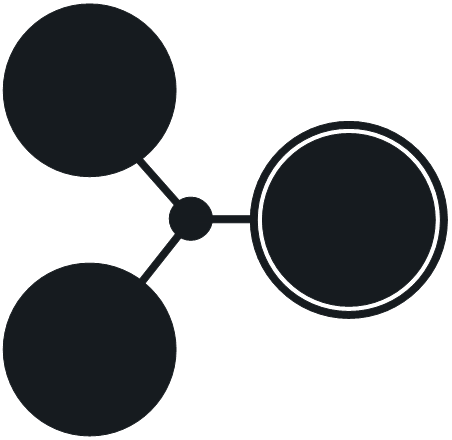
\includegraphics[width=.3\linewidth]{logo.png}\\
\vspace{20pt}
\Huge
\textbf{MOEA Framework Quick Start}\\
\vspace{20pt}
\normalsize
A Free and Open Source Java Framework for Multiobjective Optimization\\
\vspace{20pt}
\vfill
\Large{David Hadka}\\
\Large{Version %VERSION%}
\vfill
\end{center}

\end{titlepage}
% Copyright 2011-2015 David Hadka.  All Rights Reserved.
%
% This file is part of the MOEA Framework User Manual.
%
% Permission is granted to copy, distribute and/or modify this document under
% the terms of the GNU Free Documentation License, Version 1.3 or any later
% version published by the Free Software Foundation; with the Invariant Section
% being the section entitled "Preface", no Front-Cover Texts, and no Back-Cover
% Texts.  A copy of the license is included in the section entitled "GNU Free
% Documentation License".

\chapter*{}

\begin{center}

\includegraphics{gfdl.png}
\end{center}

\vspace{1em}
\noindent
Copyright 2011-2015 David Hadka.  All Rights Reserved.

\vspace{1em}
\noindent
Permission is granted to copy, distribute and/or modify this document under the terms of the GNU Free Documentation License, Version 1.3 or any later version published by the Free Software Foundation; with the Invariant Section being the section entitled ``Preface'', no Front-Cover Texts, and no Back-Cover Texts.  A copy of the license is included in the section entitled ``GNU Free Documentation License''.

\chapter*{}

\begin{center}

\includegraphics{lgpl.png}
\end{center}

\vspace{1em}
\noindent
Permission is granted to copy, distribute and/or modify the program code contained in this document under the terms of the GNU Lesser General Public License, Version 3 or any later version published by the Free Software Foundation.  Attach the following notice to any program code copied or modified from this document:

\begin{quotation}
\noindent
Copyright 2011-2015 David Hadka.  All Rights Reserved.

\vspace{1em}
\noindent
The MOEA Framework is free software: you can redistribute it and/or modify
it under the terms of the GNU Lesser General Public License as published by 
the Free Software Foundation, either version 3 of the License, or (at your 
option) any later version.

\vspace{1em}
\noindent
The MOEA Framework is distributed in the hope that it will be useful, but 
WITHOUT ANY WARRANTY; without even the implied warranty of MERCHANTABILITY 
or FITNESS FOR A PARTICULAR PURPOSE.  See the GNU Lesser General Public 
License for more details.

\vspace{1em}
\noindent
You should have received a copy of the GNU Lesser General Public License 
along with the MOEA Framework.  If not, see $<$http://www.gnu.org/licenses/$>$.
\end{quotation}

% Copyright 2011-2015 David Hadka.  All Rights Reserved.
%
% This file is part of the MOEA Framework User Manual.
%
% Permission is granted to copy, distribute and/or modify this document under
% the terms of the GNU Free Documentation License, Version 1.3 or any later
% version published by the Free Software Foundation; with the Invariant Section
% being the section entitled "Preface", no Front-Cover Texts, and no Back-Cover
% Texts.  A copy of the license is included in the section entitled "GNU Free
% Documentation License".

\chapter*{Preface}

Thank you for your interest in the MOEA Framework.  Development of the MOEA Framework started in 2009 with the idea of providing a single, consistent framework for designing, testing, and experimenting with multiobjective evolutionary algorithms (MOEAs).  In late 2011, the software was open-sourced and made available to the general public.  Since then, a large user base from the MOEA research community has formed, with thousands of users from over 112 countries.  We are indebted to the many individuals who have contributed to this project through feedback, bug reporting, code development, and testing.

As of September 2013, we have reached the next major milestone in the development and maturity of the MOEA Framework.  Version 2.0 brings with it significant changes aimed to improve both the functionality and ease-of-use of this software.  We plan to implement more algorithms within the MOEA Framework, which will improve the reliability, performance, and flexibility of the algorithms.  Doing so places the responsibility of ensuring the correctness of the MOEA implementations on our shoulders, and we will continuously work to ensure results obtained using the MOEA Framework meet the standards of scientific rigor.

We also want to reach out to the community of researchers developing new, state-of-the-art MOEAs and ask that they consider providing reference implementations of their MOEAs within the MOEA Framework.  Doing so not only disseminates your work to a wide user base, but you can take advantage of the many resources and functionality already provided by the MOEA Framework.  Please contact \mailto{contribute@moeaframework.org} if we can assist in any way.

\chapter*{Citing the MOEA Framework}

Please include a citation to the MOEA Framework in any academic publications which used or are based on results from the MOEA Framework.  For example, you can use the following in-text citation:

\begin{quote}
  \textit{This study used the MOEA Framework, version %VERSION%, available from http://www.moeaframework.org/.}
\end{quote}
% Copyright 2011-2014 David Hadka.  All Rights Reserved.
%
% This file is part of the MOEA Framework User Manual.
%
% Permission is granted to copy, distribute and/or modify this document under
% the terms of the GNU Free Documentation License, Version 1.3 or any later
% version published by the Free Software Foundation; with the Invariant Section
% being the section entitled "Preface", no Front-Cover Texts, and no Back-Cover
% Texts.  A copy of the license is included in the section entitled "GNU Free
% Documentation License".

\chapter*{Contributing to this Document}

This document is a work in progress.  Please be mindful of this fact when reading this document.  If you encounter any spelling or grammatical errors, confusing or unclear wording, inaccurate instructions, incomplete sections or missing topics, please notify us by sending an e-mail to \mailto{contribute@moeaframework.org}.  Please provide 1) the manual version number, 2) the location of the error, and 3) a description of the error.  You may alternatively send an annotated version of the PDF file.  With your help, we can provide a complete and accurate user manual for this product.

\tableofcontents

\mainmatter
% Copyright 2011-2012 David Hadka.  All Rights Reserved.
%
% This file is part of the MOEA Framework User Manual.
%
% Permission is granted to copy, distribute and/or modify this document under
% the terms of the GNU Free Documentation License, Version 1.3 or any later
% version published by the Free Software Foundation; with the Invariant Section
% being the section entitled "Preface", no Front-Cover Texts, and no Back-Cover
% Texts.  A copy of the license is included in the section entitled "GNU Free
% Documentation License".

\chapter{Introduction}


\part{Beginner's Guide - Installing and Using the MOEA Framework}
% Copyright 2011-2014 David Hadka.  All Rights Reserved.
%
% This file is part of the MOEA Framework User Manual.
%
% Permission is granted to copy, distribute and/or modify this document under
% the terms of the GNU Free Documentation License, Version 1.3 or any later
% version published by the Free Software Foundation; with the Invariant Section
% being the section entitled "Preface", no Front-Cover Texts, and no Back-Cover
% Texts.  A copy of the license is included in the section entitled "GNU Free
% Documentation License".

\chapter{Installation Instructions}

This chapter details the steps necessary to download and install the MOEA Framework on your computer.

\section{Understanding the License}

Prior to downloading, using, modifying or distributing the MOEA Framework, developers should make themselves aware of the conditions of the GNU Lesser General Public License (GNU LGPL).  While the GNU LGPL is a free software license, it does define certain conditions that must be followed in order to use, modify and distribute the MOEA Framework library.  These conditions are enacted to ensure that all recipients of the MOEA Framework (in its original and modified forms) are granted the freedoms to use, modify, study and distribute the MOEA Framework so long as the conditions of the GNU LGPL are met.  Visit \webpage{http://www.gnu.org/licenses/lgpl.html} to read the full terms of this license.

\section{Which Distribution is Right for Me?}

The MOEA Framework is currently distributed in three forms: 1) the compiled binaries; 2) the source code; and 3) the demo application.  The following text describes each distribution and its intended audience.

\paragraph{Compiled Binaries}
The compiled binaries distribution contains a fully-working MOEA Framework installation.  All required third-party libraries, data files and documentation are provided.  This download is recommended for developers integrating the MOEA Framework into an existing project.

\paragraph{Source Code}
The source code distribution contains all source code, unit tests, documentation and data files.  This distribution gives users full control over the MOEA Framework, as any component can be modified as needed.  As such, this download is recommended for developers wishing to contribute to or study the inner workings of the MOEA Framework.

\paragraph{Demo Application}
The demo application provides several interactive demos of the MOEA Framework launched by double-clicking the downloaded JAR file or running the command \plaintext{java - jar MOEAFramework-%VERSION%-Demo.jar}.  This download is intended for first-time users to quickly learn about the MOEA Framework and its capabilities.

\section{Obtaining a Copy}

The various MOEA Framework distributions can be downloaded from our website at \webpage{http://www.moeaframework.org/}.  The compiled binaries and source code distributions are packaged in a compressed tar (.tar.gz) file.  Unix/Linux/Mac users can extract the file contents using the following command:

\begin{lstlisting}[language=Plaintext]
tar -xzf MOEAFramework-%VERSION%.tar.gz
\end{lstlisting}

Windows users must use an unzip utility like 7-Zip to extract the file contents.  7-Zip is a free, open source program which can be downloaded from \webpage{http://www.7-zip.org/}.

\section{Installing Dependencies}

The software packages listed below are required or recommended in order to use the MOEA Framework.  Any software package marked as required MUST be installed on your computer in order to use the MOEA Framework.  Software marked as optional is not required to be installed, but will generally make your life easier.  This manual will often provide instructions specific to these optional software packages.

\subsection{Java 6+ (Required)}
Java 6, or any later version, is required for any system running the MOEA Framework.  If downloading the compiled binaries or demo application, you only need to install the Java Runtime Environment (JRE).  The source code download requires the Java Development Kit (JDK), which contains the compiler and other developer tools.  We recommend one of the following vendors (most are free):

\begin{description}
  \item[Oracle] - \webpage{http://www.oracle.com/technetwork/java/javase/}
    \begin{itemize}
      \item For Windows, Linux and Solaris
    \end{itemize}
    
  \item[JRockit JDK] - \webpage{http://www.oracle.com/technetwork/middleware/jrockit/}
    \begin{itemize}
      \item For Windows, Linux and Solaris
      \item May provide better performance and scalability on Intel 32 and 64-bit architectures
    \end{itemize}

  \item[OpenJDK] - \webpage{http://openjdk.java.net/}
    \begin{itemize}
      \item For Ubuntu 8.04 (or later), Fedora 9 (or later), Red Hat Enterprise Linux 5, openSUSE 11.1, Debian GNU/Linux 5.0 and OpenSolaris
    \end{itemize}

  \item[IBM] - \webpage{http://www.ibm.com/developerworks/java/jdk/}
    \begin{itemize}
      \item For AIX, Linux and z/OS
    \end{itemize}
  \item[Apple] - \webpage{http://support.apple.com/kb/DL1572}
\end{description}

Please follow the installation instruction accompanying your chosen JRE or JDK.

\subsection{Eclipse or NetBeans (Optional)}
Eclipse and NetBeans are two development environments for writing, debugging, testing, and running Java programs.  Eclipse can be downloaded for free from \webpage{http://www.eclipse.org/}, and NetBeans can be obtained from \webpage{http://netbeans.org/}.

The installation of Eclipse is simple --- just extract the compressed file to a folder of your choice and run the Eclipse executable from this folder.  First-time users of Eclipse may be prompted to select a workspace location.  The default location is typically fine.  Click the checkbox to no longer show this dialog and click Ok.

To install NetBeans, simply run the executable.  Once installed, you can launch NetBeans by clicking the NetBeans link in your start menu.

\subsection{Apache Ant (Optional)}
Apache Ant is a Java tool for automatically compiling and packaging projects, similar to the Make utility on Unix/Linux.  Individuals working with the source code distribution should consider installing Apache Ant, as it helps automate building and testing the MOEA Framework.  Apache Ant can be downloaded from \webpage{http://ant.apache.org/}.  The installation instructions provided by Ant should be followed.

Note that Eclipse contains Ant, so it is not necessary to install Eclipse and Ant together.

\section{Importing into Eclipse}
When working with the source code distribution, it is necessary to properly configure the Java environment to ensure all resources are available.  To assist in this process, the source code distribution includes the necessary files to import directly into Eclipse.

To import the MOEA Framework project into Eclipse, first start Eclipse and select File $\rightarrow$ Import... from the menu.  A popup window will appear.  Ensure the General $\rightarrow$ Existing Projects into Workspace item is selected and click Next.  A new window will appear.  In this new window, locate the Set Root Directory entry.  Using the Browse button, select the \folder{\moeaframework} folder containing the source code.  Finally, click Finish.  The MOEA Framework will now be properly configured in Eclipse.

\section{Importing into NetBeans}
If you downloaded the source code, you can import the MOEA Framework into NetBeans as follows.  In NetBeans, select New Project from the File menu.  In the screen that appears, select the ``Java'' category and ``Java Project with Existing Sources''.  Click Next.

Specify the project name as ``MOEA Framework''.  Set the project folder by clicking the Browse button and selecting the \folder{\moeaframework} folder.  Click Next.

Add the \folder{src} and \folder{examples} folders as Source Package Folders.  Click Finish.  The MOEA Framework project should now appear in the Projects window.

Finally, we need to add the third-party libraries used by the MOEA Framework.  Right-click the MOEA Framework project in the Projects window and select Properties.  In the window that appears, click Libraries in the left-hand panel.  On the right-side of the window, click the button ``Add Jars/Folder''.  Browse to the \folder{\moeaframework/lib} folder, highlight all the JAR files (using shift or alt to select multiple files), and click Ok.  Be sure that you select each individual JAR file and not the folder containing the JAR files.  Click the ``Add Jars/Folder'' button again.  Navigate to and select the root \folder{\moeaframework} folder, and click Ok.  You should now see $8$ items in the compile-time libraries list.  There should be $7$ entries referencing \plaintext{.jar} files the ``\folder{.}'' as the last entry.  Your screen should look like \figref{fig:netbeans}.  Click Ok when finished.

\begin{figure}
  \center
  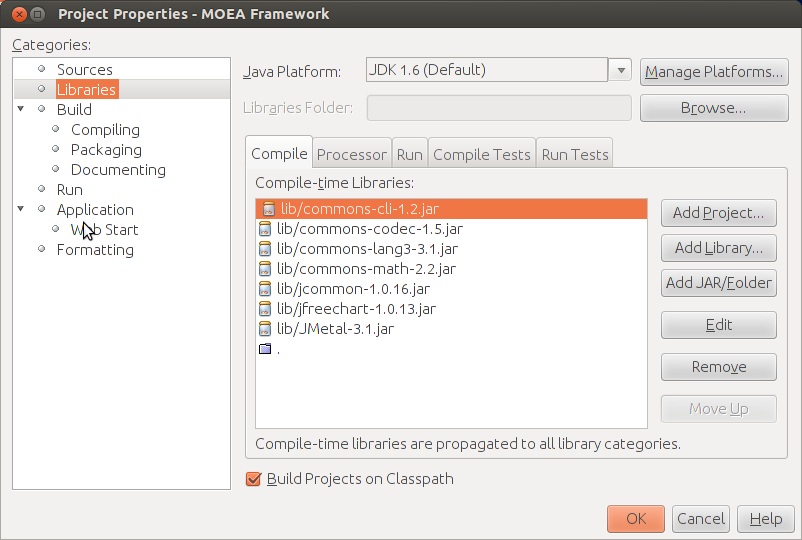
\includegraphics[width=.8\linewidth]{netbeans.png}
  \caption{How the NetBeans properties window should appear in the MOEA Framework is properly configured.}
  \label{fig:netbeans}
\end{figure}

Test your NetBeans install by running Example1.  You can run an example by expanding the \folder{examples} folder in the Project window, right-clicking Example1, and selecting Run File from the popup menu.

\section{Testing your Installation}
Having finished installing the MOEA Framework and its dependencies, it is useful to run the MOEA Diagnostic Tool to test if the installation was successful.  If the diagnostic tool appears and you can run any algorithm, then the installation was successful.

\paragraph{Compiled Binaries}
Run the launch-diagnostic-tool.bat file on Windows.  You can manually run the diagnostic tool with the following command:

\begin{lstlisting}[language=Plaintext]
java -Djava.ext.dirs=lib
		org.moeaframework.analysis.diagnostics.LaunchDiagnosticTool
\end{lstlisting}

\paragraph{Source Code}
Inside Eclipse, navigate to the src $\rightarrow$ org $\rightarrow$ moeaframework $\rightarrow$ analysis $\rightarrow$ diagnostic package in the Package Explorer window.  Right-click the file \texttt{LaunchDiagnosticTool.java} and select the Run as $\rightarrow$ Java Application option in the popup menu.

\paragraph{Demo Program}
Double-click the downloaded JAR file.  If the demo window does not appear, try to manually launch the tool with with the following command:

\begin{lstlisting}[language=Plaintext]
java -jar MOEAFramework-%VERSION%-Demo.jar
\end{lstlisting}

\section{Distribution Contents}
This section describes the contents of the compiled binaries and source code distribution downloads.

\subsection{Compiled Binary Contents}
\begin{description}
  \item[\folder{javadoc/}] contains the MOEA Framework API, which is a valuable resource for software developers as it provides descriptions of all classes, methods and variables available in the MOEA Framework.  The API may be viewed in a web browser by opening the \file{index.html} file.
  \item[\folder{lib/}] contains the compiled libraries required to use the MOEA Framework.  This includes the MOEA Framework compiled libraries and all required third-party libraries.
  \item[\folder{licenses/}] contains the complete text of all open source software licenses for the MOEA Framework and third-party libraries.  In order to comply with the licenses, this folder should always be distributed alongside the compiled libraries in the lib folder.
  \item[\folder{pf/}] contains the Pareto front files for the test problems provided by default in the MOEA Framework.
  \item[\file{global.properties}] is the configuration file for the MOEA Framework.  Default settings are used unless the settings are provided in this file.
  \item[\file{HELP}] provides a comprehensive list of errors and warning messages encountered when using the MOEA Framework.  When available, information about the cause and ways to fix errors are suggested.
  \item[\file{launch-diagnostic-tool.bat}] launches the diagnostic tool GUI that allows users to run algorithms and display runtime information about the algorithms.  This file is for Windows systems only.
  \item[\file{LICENSE}] lists the open source software licenses in use by the MOEA Framework, contributor code and third-party libraries.
  \item[\file{NEWS}] details all important changes made in the current release and prior releases.  This includes critical bug fixes, changes, enhancements and new features.
  \item[\file{README}] provides information about obtaining, installing, using, distributing, licensing and contributing to the MOEA Framework.
\end{description}

\subsection{Source Code Contents}
\begin{description}
  \item[\folder{auxiliary/}] contains an assortment of files and utilities used by the MOEA Framework, but are not required in a build.  For instance, this folder contains example C/C++ code for interfacing C/C++ problems with the MOEA Framework.
  \item[\folder{examples/}] contains examples using the MOEA Framework.  These examples are also available on the website.
  \item[\folder{lib/}] contains all required third-party libraries used by the MOEA Framework.
  \item[\folder{manual/}] contains the LaTeX files and figures for generating this user manual.
  \item[\folder{META-INF/}] contains important files which are packaged with the compiled binaries.  Such files include the service provider declarations, licensing information, etc.
  \item[\folder{pf/}] contains the Pareto front files for the test problems provided by default in the MOEA Framework.
  \item[\folder{src/}] contains all source code in use by the core MOEA Framework library.
  \item[\folder{test/}] contains all JUnit unit tests used to ensure the correctness of the MOEA Framework source code.
  \item[\folder{website/}] contains all files used to generate the website.
  \item[\file{build.xml}] contains the Apache Ant build scripts for compiling and/or building the MOEA Framework library.
  \item[\file{global.properties}] is the configuration file for the MOEA Framework.  Default settings are used unless the settings are provided in this file.
  \item[\file{HELP}] provides a comprehensive list of errors and warning messages encountered when using the MOEA Framework.  When available, information about the cause and ways to fix errors are suggested.
  \item[\file{LICENSE}] lists the open source software licenses in use by the MOEA Framework, contributor code and third-party libraries.
  \item[\file{NEWS}] details all important changes made in the current release and prior releases.  This includes critical bug fixes, changes, enhancements and new features.
  \item[\file{README}] provides information about obtaining, installing, using, distributing, licensing and contributing to the MOEA Framework.
  \item[\file{test.xml}] contains the Apache Ant testing scripts used to automatically run all JUnit unit tests and provide a human-readable report of the test results.
  \item[\file{TODO}] lists all planned changes for the MOEA Framework source code.  This file is a starting point for individuals wishing to contribute modifications to the MOEA Framework.
\end{description}

\section{Resolving Dependencies with Maven}
As of version 2.4, the MOEA Framework and its dependencies can be resolved using the Maven dependency management system.  Maven is available from \webpage{http://maven.apache.org/}.  To add the MOEA Framework to your Maven project, add the following dependency to your \file{pom.xml} file:

\begin{lstlisting}[language=Plaintext]
<dependency>
	<groupId>org.moeaframework</groupId>
	<artifactId>moeaframework</artifactId>
	<version>%VERSION%</version>
</dependency>
\end{lstlisting}

\section{Conclusion}
This chapter described each of the MOEA Framework distributions.  At this point, you should have a working MOEA Framework distribution which you can use to run the examples in subsequent chapters.
% Copyright 2011-2013 David Hadka.  All Rights Reserved.
%
% This file is part of the MOEA Framework User Manual.
%
% Permission is granted to copy, distribute and/or modify this document under
% the terms of the GNU Free Documentation License, Version 1.3 or any later
% version published by the Free Software Foundation; with the Invariant Section
% being the section entitled "Preface", no Front-Cover Texts, and no Back-Cover
% Texts.  A copy of the license is included in the section entitled "GNU Free
% Documentation License".

\chapter{Executor, Instrumenter, Analyzer}

The Executor, Instrumenter and Analyzer classes provide most of the functionality provided by the MOEA Framework.  This chapter walks through several introductory examples using these classes.

\section{Executor}
The Executor class is responsible for constructing and executing runs of an algorithm.  A single run requires three pieces of information: 1) the problem; 2) the algorithm used to solve the problem; and 3) the number of objective function evaluations allocated to solve the problem.  The following code snippet demonstrates how these three pieces of information are passed to the Executor.

\begin{lstlisting}[language=Java]
NondominatedPopulation result = new Executor()
		.withProblem("UF1")
		.withAlgorithm("NSGAII")
		.withMaxEvaluations(10000)
		.run();
\end{lstlisting}

Line 1 creates a new Executor instance.  Lines 2, 3 and 4 set the problem, algorithm and maximum number of objective function evaluations, respectively.  In this example, we are solving the two-objective UF1 test problem using the NSGA-II algorithm.  Lastly, line 5 runs this experiment and returns the resulting approximation set.

Note how, on lines 2 and 3, the problem and algorithm are specified using strings.  There exist a number of pre-defined problems and algorithms which are available in the MOEA Framework.  Furthermore, the MOEA Framework can be easily extended to provide additional problems and algorithms which can be instantiated in a similar manner.

Once the run is complete, we can access the result.  Line 1 above shows that the approximation set, which is a \texttt{NondominatedPopulation}, gets assigned to a variable named result.  This approximation set contains all Pareto optimal solutions produced by the algorithm during the run.  For example, the code snippet below prints out the two objectives to the console.

\begin{lstlisting}[language=Java]
for (Solution solution : result) {
	System.out.println(solution.getObjective(0) + " " +
			solution.getObjective(1));
}
\end{lstlisting}

Line 1 loops over each solution in the result.  A solution stores the decision variables, objectives, constraints and any relevant attributes.  Lines 2 and 3 demonstrate how the objective values can be retrieved from a solution.

Putting all this together and adding the necessary boilerplate Java code, the complete code snippet is shown below.

\begin{lstlisting}[language=Java]
import java.util.Arrays;
import org.moeaframework.Executor;
import org.moeaframework.core.NondominatedPopulation;
import org.moeaframework.core.Solution;

public class Example1 {

	public static void main(String[] args) {
		NondominatedPopulation result = new Executor()
				.withProblem("UF1")
				.withAlgorithm("NSGAII")
				.withMaxEvaluations(10000)
				.run();

		for (Solution solution : result) {
			System.out.println(solution.getObjective(0) 
					+ " " + solution.getObjective(1));
		}
	}

}
\end{lstlisting}

Since line 6 defines the class name to be \texttt{Example1}, this code snippet must be saved to the file \file{Example1.java}.  Compiling and running this file will produce output similar to:

\begin{lstlisting}[language=Plaintext]
0.44231379762506046 0.359116256460771
0.49221581122496827 0.329972177772519
0.8024234727753593 0.11620643510507386
0.7754123383456428 0.14631335018878214
0.4417794310706653 0.3725544250337767
0.11855110357018901 0.6715178312971422
...
\end{lstlisting}

The \texttt{withProblem} and \texttt{withAlgorithm} methods allow us to specify the problem and algorithm by name.  Changing the problem or algorithm is as simple as changing the string passed to these methods.  For example, replacing line 11 in the code snippet above to \java{withAlgorithm("GDE3")} will now allow you to run the Generalized Differential Evolution 3 (GDE3) algorithm.  Most existing MOEA libraries require users to instantiate and configure each algorithm manually.  In the MOEA Framework, such details are handled by the Executor.

The MOEA Framework is distributed with a number of built-in problems and algorithms.  See the API documentation for \texttt{StandardProblems} and \texttt{StandardAlgorithms} to see the list of problems and algorithms available, respectively.  This documentation is available online at \webpage{http://www.moeaframework.org/javadoc/org/moeaframework/problem/StandardProblems.html} and \webpage{http://www.moeaframework.org/javadoc/org/moeaframework/algorithm/StandardAlgorithms.html}.

When specifying only the problem, algorithm and maximum evaluations, the Executor assumes default parameterizations for the internal components of the algorithm.  For instance, NSGA-II parameters include the population size, the simulated binary crossover (SBX) rate and distribution index, and the polynomial mutation (PM) rate and distribution index.  Changing the parameter settings from their defaults is possible using the \texttt{setProperty} methods.  Each parameter is identified by a key and is assigned a numeric value.  For example, all of NSGA-II's parameters are set in the following code snippet:

\begin{lstlisting}[language=Java]
NondominatedPopulation result = new Executor()
		.withProblem("UF1")
		.withAlgorithm("NSGAII")
		.withMaxEvaluations(10000)
		.withProperty("populationSize", 50)
		.withProperty("sbx.rate", 0.9)
		.withProperty("sbx.distributionIndex", 15.0)
		.withProperty("pm.rate", 0.1)
		.withProperty("pm.distributionIndex", 20.0)
		.run();
\end{lstlisting}

Each algorithm defines its own parameters.  Refer to the API documentation for the exact parameter keys.  Any parameters not explicitly defined using the \texttt{withProperty} methods will be set to their default values.

The Executor also provides some more advanced features.  First, it contains several methods for distributing objective function evaluations across multiple processing cores or computers.  Distributing evaluations can significantly speed up a run through parallelization.  The simplest way to enable parallelization is through the \texttt{distributeOnAllCores} method.  This will distribute objective function evaluations across all cores on your local computer.  Note that not all algorithms can support parallelization.  In such cases, the MOEA Framework will still run the algorithm, but it will not be parallelized.

Second, the MOEA Framework provides checkpointing functionality.  As an algorithm is running, checkpoint files will be periodically saved.  The checkpoint file stores the current state of the algorithm.  If the run is interrupted, such as during a power outage, the run can be resumed at the last saved checkpoint.  The \texttt{setCheckpointFile} sets the file location for the checkpoint file, and \texttt{checkpointEveryIteration} or \texttt{setCheckpointFrequency} control how frequently the checkpoint file is saved.

Resuming a run from a checkpoint occurs automatically.  If the checkpoint file does not exist, a run starts from the beginning.  However, if the checkpoint file exists, then the run is automatically resumed at that checkpoint.

\begin{tip}
Care must be taken when using checkpoints as they can be a source of confusion for new users.  For instance, using the same checkpoint file from an unrelated run can cause unexpected behavior or an error.  For this reason, checkpoints are recommended only when solving time-consuming problems.
\end{tip}

The snippet below extends our example with distributed evaluations and checkpointing.  In addition to the code below, you will need to import the \java{File} class by adding \java{import java.io.File} at the beginning of the file.

\begin{lstlisting}[language=Java]
NondominatedPopulation result = new Executor()
		.withProblem("UF1")
		.withAlgorithm("NSGAII")
		.withMaxEvaluations(10000)
		.withProperty("populationSize", 50)
		.withProperty("sbx.rate", 0.9)
		.withProperty("sbx.distributionIndex", 15.0)
		.withProperty("pm.rate", 0.1)
		.withProperty("pm.distributionIndex", 20.0)
		.distributeOnAllCores()
		.checkpointEveryIteration()
		.withCheckpointFile(new File("UF1_NSGAII.chkpt"))
		.run();
\end{lstlisting}

\begin{important}
Checkpoint files are never deleted by the MOEA Framework.  Each time you run this example, it will resume from its last save point.  If you want to run this example from the beginning, you must delete the checkpoint file manually.  In this example, the checkpoint file is saved in the \folder{\moeaframework} folder.
\end{important}

\section{Instrumenter}
In addition to supporting a multitude of algorithms and test problems, the MOEA Framework also contains a comprehensive suite of tools for analyzing the performance of algorithms.  The MOEA Framework supports both run-time dynamics and end-of-run analysis.  Run-time dynamics capture the behavior of an algorithm throughout the duration of a run, recording how its solution quality and other elements change.  End-of-run analysis, on the other hand, focuses on the result of a complete run and comparing the relative performance of various algorithms.  Run-time dynamics will be introduced in this section using the Instrumenter; end-of-run analysis will be discussed in the following section using the Analyzer.

The Instrumenter gets its name from its ability to add instrumentation, which are pieces of code that record information, to an algorithm.  A range of data can be collected using the Instrumenter, including:

\begin{enumerate}
  \item Elapsed time
  \item Population size / archive size
  \item The approximation set
  \item Performance metrics
  \item Restart frequency
\end{enumerate}

The Instrumenter works hand-in-hand with the Executor to collect its data.  The Executor is responsible for configuring and running the algorithm, but it allows the Instrumenter to record the necessary data while the algorithm is running.  To start collecting run-time dynamics, we first create and configure an Instrumenter instance.

\begin{lstlisting}[language=Java]
Instrumenter instrumenter = new Instrumenter()
		.withProblem("UF1")
		.withFrequency(100)
		.attachAll();
\end{lstlisting}

First, line 1 creates the new Instumenter instance.  Next, line 2 specifies the problem.  This allows the instrumenter to access the known reference set for this problem, which is necessary for evaluating performance metrics.  Third, line 3 sets the frequency at which the data is recorded.  In this example, data is recorded every 100 evaluations.  Lastly, line 4 indicates that all available data should be collected.

Next, we create and configure the Executor instance with the following code snippet:

\begin{lstlisting}[language=Java]
NondominatedPopulation result = new Executor()
		.withProblem("UF1")
		.withAlgorithm("NSGAII")
		.withMaxEvaluations(10000)
		.withInstrumenter(instrumenter)
		.run();
\end{lstlisting}

This code snippet is similar to the previous examples of the Executor, but includes the addition of line 5.  Line 5 tells the executor that all algorithms it executes will be instrumented with our Instrumenter instance.  Once the instrumenter is set and the algorithm is configured, we can run the algorithm on line 6.

When the run completes, we can access the data collected by the instrumenter.  The data is stored in an Accumulator object.  The Accumulator for the run we just executed can be retrieved with the following line:

\begin{lstlisting}[language=Java]
Accumulator accumulator = instrumenter.getLastAccumulator();
\end{lstlisting}

An Accumulator is similar to a Map in that it stores key-value pairs.  The key identifies the type of data recorded.  However, instead of storing a single value, the Accumulator stores many values, one for each datapoint collected by the Instrumenter.  Recall that in this example, we are recording a datapoint every 100 evaluations (i.e., the frequency).  The data can be extracted from an Accumulator with a loop similar to the following:

\begin{lstlisting}[language=Java]
for (int i=0; i<accumulator.size("NFE"); i++) {
	System.out.println(accumulator.get("NFE", i) + "\t" +  
			accumulator.get("GenerationalDistance", i));
}
\end{lstlisting}

In this code snippet, we are printing out two columns of data: the number of objective function evaluations (NFE) and the generational distance performance indicator.  Including all the boilerplate Java code, the complete example is provided below.

\begin{lstlisting}[language=Java]
import java.io.IOException;
import java.io.File;
import org.moeaframework.core.NondominatedPopulation;
import org.moeaframework.Instrumenter;
import org.moeaframework.Executor;
import org.moeaframework.analysis.collector.Accumulator;

public class Example2 {

	public static void main(String[] args) throws IOException {
		Instrumenter instrumenter = new Instrumenter()
				.withProblem("UF1")
				.withFrequency(100)
				.attachAll();

		NondominatedPopulation result = new Executor()
				.withProblem("UF1")
				.withAlgorithm("NSGAII")
				.withMaxEvaluations(10000)
				.withInstrumenter(instrumenter)
				.run();

		Accumulator accumulator = instrumenter.getLastAccumulator();

		for (int i=0; i<accumulator.size("NFE"); i++) {
			System.out.println(accumulator.get("NFE", i) + "\t" +  
					accumulator.get("GenerationalDistance", i));
		}
	}

}
\end{lstlisting}

Since line 8 defines the class name to be \texttt{Example2}, this code snippet must be saved to the file \file{Example2.java}.  Compiling and running this file will produce output similar to:

\begin{lstlisting}[language=Plaintext]
100    0.6270289757162074
200    0.5843583367503041
300    0.459146246330144
400    0.36799025371209954
500    0.3202295846482732
600    0.2646381449859231
...
\end{lstlisting}

This shows how NSGA-II experiences rapid convergence early in a run.  In the first 600 evaluations, the generational distance decreases to 33\% of its starting value.  Running for longer, you should see the speed of convergence begin to level off.  This type of curve is commonly seen when using MOEAs.  They often experience a rapid initial convergence that quickly levels off.  You can confirm this behavior by running this example on different algorithms.

\begin{tip}
There are a few things to keep in mind when using the Instrumenter. First, instrumenting an algorithm and recording all the data will slow down the execution of algorithms and significantly increase their memory usage.  For this reason, we strongly recommend limiting the data collected to what you consider important.  To limit the data collected, simply replace the \texttt{attachAll} method with one or more specific attach methods, such as \texttt{attachGenerationalDistanceCollector}.  Changing the collection frequency is another way to reduce the performance and memory usage.
\end{tip}

Second, if the memory usage exceeds that which is allocated to Java, you will receive an \texttt{OutOfMemoryException}.  The immediate solution is to increase the amount of memory allocated to Java by specifying the \texttt{-Xmx} command-line option when starting a Java application.  For example, the following command will launch a Java program with 512 MBs of available memory.

\begin{quote}
  \texttt{java -Xmx512m ...rest of command...}
\end{quote}

If you have set the \texttt{-Xmx} option to include all available memory on your computer and you still receive an \texttt{OutOfMemoryException}, then you need to decrease the collection frequency or restrict what data is collected.

Third, the Instrumenter only collects data which is provided by the algorithm.  For instance, an Instrumenter with \texttt{attachAdaptiveTimeContinuationCollector} will work perfectly fine on an algorithm that does support adaptive time continuation.  The Instrumenter examines the composition of the algorithm and only collects data for the components it finds.  This also implies that the Instrumenter will work on any algorithm, including any provided by third-party providers.

\section{Analyzer}
The Analyzer provides end-of-run analysis.  This analysis focuses on the resulting Pareto approximation set and how it compares against a known reference set.  The Analyzer is particularly useful for statistically comparing the results produced by two or more algorithms, or possibly the same algorithm with different parameter settings.  To start using the Analyzer, we first create and configure a new instance, as shown below.

\begin{lstlisting}[language=Java]
Analyzer analyzer = new Analyzer()
		.withProblem("UF1")
		.includeAllMetrics()
		.showStatisticalSignificance();
\end{lstlisting}

First, we construct a new Analyzer on line 1.  Next, on line 2 we set the problem in the same manner as required by the Executor and Instrumenter.  Line 3 tells the Analyzer to evaluate all available performance metrics.  Lastly, line 4 enables the statistical comparison of the results.

Next, the code snippet below shows how the Executor is used to run NSGA-II and GDE3 for 50 replications and store the results in the Analyzer.  Running for multiple replications, or seeds, is important when generating statistical results.

\begin{lstlisting}[language=Java]
Executor executor = new Executor()
		.withProblem("UF1")
		.withMaxEvaluations(10000);

analyzer.addAll("NSGAII",  
		executor.withAlgorithm("NSGAII").runSeeds(50));

analyzer.addAll("GDE3",
		executor.withAlgorithm("GDE3").runSeeds(50));
\end{lstlisting}

Lines 1-3 create the Executor, similar to the previous examples except we do not yet specify the algorithm.  Lines 5-6 run NSGA-II.  Note how we first set the algorithm to NSGA-II, run it for 50 seeds, and add the results from the 50 seeds to the analyzer.  Similarly, on lines 8-9 we run GDE3 and add its results to the analyzer.  Note how lines 5 and 8 pass a string as the first argument to \texttt{addAll}.  This gives a name to the samples collected, which can be any string and not necessarily the algorithm name as is the case in this example.

Lastly, we can display the results of the analysis with the following line.

\begin{lstlisting}[language=Java]
analyzer.printAnalysis();
\end{lstlisting}

Putting all of this together and adding the necessary boilerplate Java code results in:

\begin{lstlisting}[language=Java]
import java.io.IOException;
import org.moeaframework.Analyzer;
import org.moeaframework.Executor;

public class Example3 {

	public static void main(String[] args) throws IOException {
		Analyzer analyzer = new Analyzer()
				.withProblem("UF1")
				.includeAllMetrics()
				.showStatisticalSignificance();

		Executor executor = new Executor()
				.withProblem("UF1")
				.withMaxEvaluations(10000);

		analyzer.addAll("NSGAII",  
				executor.withAlgorithm("NSGAII").runSeeds(50));

		analyzer.addAll("GDE3",
				executor.withAlgorithm("GDE3").runSeeds(50));

		analyzer.printAnalysis();
	}

}
\end{lstlisting}

The output of which will look similar to:

\begin{lstlisting}[language=Plaintext]
GDE3:
    Hypervolume:
        Min: 0.4358713988821755
        Median: 0.50408587891491
        Max: 0.5334024567416756
        Count: 50
        Indifferent: []
...
NSGAII:
    Hypervolume:
        Min: 0.3853879478063566
        Median: 0.49033837779756184
        Max: 0.5355927774923894
        Count: 50
        Indifferent: []
...
\end{lstlisting}

Observe how the results are organized by the indenting.  It starts with the sample names, GDE3 and NSGAII in this example.  The first indentation level shows the different metrics, such as Hypervolume.  The second indentation level shows the various statistics for the metric, such as the minimum, median and maximum values.

The indifferent field show the statistical significance of the results.  The Analyzer applies the Mann-Whitney and Kruskal-Wallis tests for statistical significance.  If the medians are significantly different, then the indifferent columns shows empty brackets (i.e., \texttt{[]}).  However, if the medians are indifferent, then the samples which are indifferent will be shown within the brackets.  For example, if GDE3's indifferent field was \texttt{[NSGAII]}, then that indicates there is no statistical difference in performance between GDE3 and NSGA-II.

Statistical significance is important when comparing multiple algorithms, particularly when the results will be reported in scientific papers.  Running an algorithm will likely produce different results each time it is run.  This is because many algorithms are stochastic (meaning that they include sources of randomness).  Because of this, it is a common practice to run each algorithm for multiple seeds, with each seed using a different random number sequence.  As a result, an algorithm does not produce a single result.  It produces a distribution of results.  When comparing algorithms based on their distributions, it is necessary to use statistical tests.  Statistical tests allow us to determine if two distributions (i.e., two algorithms) are similar or different.  This is exactly what is provided when enabling \texttt{showStatisticalSignificance} and viewing the Indifferent entries in the output from Analyzer.

In the example above, we called \texttt{includeAllMetrics} to include all performance metrics in the analysis.  This includes hypervolume, generational distance, inverted generational distance, spacing, additive $\epsilon$-indicator, maximum Pareto front error and reference set contribution.  It is possible to enable specific metrics by calling their corresponding include method, such as \texttt{includeGenerationalDistance}.

\section{Conclusion}
This chapter introduced three of the high-level classes: the Executor, Instrumenter and Analyzer.  The examples provided show the basics of using these classes, but their functionality is not limited to what was demonstrated.  Readers should explore the API documentation for these classes to discover their more sophisticated functionality.
% Copyright 2011-2013 David Hadka.  All Rights Reserved.
%
% This file is part of the MOEA Framework User Manual.
%
% Permission is granted to copy, distribute and/or modify this document under
% the terms of the GNU Free Documentation License, Version 1.3 or any later
% version published by the Free Software Foundation; with the Invariant Section
% being the section entitled "Preface", no Front-Cover Texts, and no Back-Cover
% Texts.  A copy of the license is included in the section entitled "GNU Free
% Documentation License".

\chapter{Defining New Problems}
\label{chpt:problems}

The real value of the MOEA Framework comes not from the algorithms and tools it provides, but the problems that it solves.  As such, being able to introduce new problems into the MOEA Framework is an integral aspect of its use.

Throughout this chapter, we will show how a simple multiobjective problem, the Kursawe problem, can be defined in Java, C/C++, and in scripting languages.  The formal definition for the Kursawe problem is provided below.

\begin{equation}
  \label{eq:mop}
  \begin{aligned}
    & \underset{\vect{x} \in \mathbb{R}^L}{\text{minimize}}
      & & F(\vect{x}) = (f_1(\vect{x}), f_2(\vect{x})) \\
    & \text{where}
      & & f_1(\vect{x}) = \sum_{i=0}^{L-1} -10\text{e}^{-0.2\sqrt{x_i^2 + x_{i+1}^2}}, \\
    & & & f_2(\vect{x}) = \sum_{i=0}^{L} \left|x_i\right|^{0.8} + 5\sin\left(x_i^3\right).
  \end{aligned}
\end{equation}

\begin{important}
The MOEA Framework only works on minimization problems.  If any objectives in your problem are to be maximized, you can negate the objective value to convert from maximization into minimization.  In other words, by minimizing the negated objective, your are maximizing the original objective.  See section \ref{sect:maximizing} for additional details on dealing with maximization objectives.
\end{important}

\section{Java}
Defining new problems in Java is the most direct and straightforward way to introduce new problems into the MOEA Framework.  All problems in the MOEA Framework implement the \class{Problem} interface.  The \class{Problem} interface defines the methods for characterizing a problem, defining the problem's representation, and evaluating solutions to the problem.  In practice, you should never need to implement the \class{Problem} interface directly, but can extend the more convenient \class{AbstractProblem} class.  \class{AbstractProblem} provides default implementations for many of the methods required by the \class{Problem} interface.  The code example below shows the Kursawe problem defined by extending the \class{AbstractProblem} class.

\begin{lstlisting}[language=Java]
import org.moeaframework.core.Solution;
import org.moeaframework.core.variable.EncodingUtils;
import org.moeaframework.core.variable.RealVariable;
import org.moeaframework.problem.AbstractProblem;
 
public class Kursawe extends AbstractProblem {
 
	public Kursawe() {
		super(3, 2);
	}

	@Override
	public Solution newSolution() {
		Solution solution = new Solution(numberOfVariables, 
				numberOfObjectives);
 
		for (int i = 0; i < numberOfVariables; i++) {
			solution.setVariable(i, new RealVariable(-5.0, 5.0));
		}
 
		return solution;
	}

	@Override
	public void evaluate(Solution solution) {
		double[] x = EncodingUtils.getReal(solution);
		double f1 = 0.0;
		double f2 = 0.0;
   	 
		for (int i = 0; i < numberOfVariables - 1; i++) {
			f1 += -10.0 * Math.exp(-0.2 * Math.sqrt(
					Math.pow(x[i], 2.0) + Math.pow(x[i+1], 2.0)));
		}
 
		for (int i = 0; i < numberOfVariables; i++) {
			f2 += Math.pow(Math.abs(x[i]), 0.8) +  
					5.0 * Math.sin(Math.pow(x[i], 3.0));
		}
 
		solution.setObjective(0, f1);
		solution.setObjective(1, f2);
	}
 
}
\end{lstlisting}

Note on line 9 in the constructor, we call \java{super(3, 2)} to set the number of decision variables (3) and number of objectives (2).  All that remains is defining the \java{newSolution} and \java{evaluate} methods.

The \java{newSolution} method is responsible for instantiating new instances of solutions for the problem, and in doing so defines the decision variable types and bounds.  In the \java{newSolution} method, we start by creating a new \class{Solution} instance on lines 14-15.  Observe that we must pass the number of decision variables and objectives to the \class{Solution} constructor.  Next, we define each of the decision variables and specify their bounds on lines 17-19.  For the Kursawe problem, all decision variables are real values ranging between $-5.0$ and $5.0$, inclusively.  Finally, we complete this method by returning the \class{Solution} instance.

The \java{evaluate} method is responsible for evaluating solutions to the problem.  A solution which has been generated by an optimization algorithm is passed as an argument to the \java{evaluate} method.  The decision variables contained in this solution are set to the values specified by the optimization algorithm.  The evaluate method must extract these values, evaluate the problem, and set the objective values.

Since the Kursawe problem contains all real-valued decision variables, we can cast the decision variables to an array using the helpful methods of the \class{EncodingUtils} class on line 26.  Use of \class{EncodingUtils} is encouraged for extracting the decision variables from a solution.  Then on lines 27 to 38, we use those decision variables to evaluate the Kursawe problem.  Finally, on lines 40-41, we assign the two objectives for this problem.

At this point, the problem is completely defined and can be used with the MOEA Framework.  The following section describes how to reference user-defined problems within the MOEA Framework.

\section{Referencing the Problem}
Once a new problem is defined in Java, it can be referenced by the MOEA Framework in a number of ways.  This section details the various methods for referencing problems.

\subsection{By Class}
The \class{Executor}, \class{Instrumenter} and \class{Analyzer} classes introduced in \chptref{chpt:executor} all accept direct references to the problem class using the \java{withProblemClass} method.  For example, following the previous example with the Kursawe problem, we can optimize this problem with the following code:

\begin{lstlisting}[language=Java]
new Executor()
		.withProblemClass(Kursawe.class)
		.withAlgorithm("NSGAII")
		.withMaxEvaluations(10000)
		.run();
\end{lstlisting}

Note how the Kursawe problem is specified by name followed by \java{.class}.  This passes a direct reference to the Kursawe class we created in the previous chapter.

Problems can also define constructors with arguments.  For example, consider a problem that needs to load data from a file.  For this to work, define a constructor in the problem class that accepts the desired inputs.  In this case, our constructor would be called \java{public ProblemWithArgument(File dataFile) { ... }}.  You can then solve this problem as shown below.

\begin{lstlisting}[language=Java]
new Executor()
		.withProblemClass(ProblemWithArgument.class, new File("inputFile.txt"))
		.withAlgorithm("NSGAII")
		.withMaxEvaluations(10000)
		.run();
\end{lstlisting}

\subsection{By Class Name}
As of version 1.11, problems can be referenced by their fully-qualified class name.  The fully-qualified class name includes the Java package in which the class is defined.  For example, the Schaffer problem's fully-qualified class name is \classpath{org.moeaframework.problem.misc.Schaffer}.  The problem \emph{must} have an empty (no argument) constructor.

The class name can be used to run problems anywhere the MOEA Framework accepts a string representation of the problem.  This includes but is not limited to
\begin{enumerate}
  \item The \java{withProblem} method in \class{Executor}, \class{Instrumenter} and \class{Analyzer}
  \item Any command line utilities with a problem argument
  \item The problem selection combo box in the MOEA Diagnostic Tool
\end{enumerate}

\subsection{By Name}

The MOEA Framework also provides the option to reference problems by name.  There are two advantages to using this approach.  First, this approach allows the use of short, meaningful names.  For example, rather than specifying the fully-qualified class name for the Schaffer problem, \classpath{org.moeaframework.problem.misc.Schaffer}, one can use the name \class{Schaffer} instead.  Second, a reference set for named problems can optionally be defined.  This reference set will be automatically used wherever a reference set is required.  Without this, a reference set must be manually specified by the user or programmer each time it is required.

The disadvantage to this approach is that some additional configuration is necessary to provide the mapping from the problem name to the problem class.  As such, this approach is recommended for third-party library developers who are developing new problems to be used with the MOEA Framework.  The remainder of this section describes two such methods for referencing problems by name.

The problem name can be used to run problems anywhere the MOEA Framework accepts a string representation of the problem.  This includes but is not limited to
\begin{enumerate}
  \item The \texttt{withProblem} method in \class{Executor}, \class{Instrumenter} and \class{Analyzer}
  \item Any command line utilities with a problem argument
  \item The problem selection combo box in the MOEA Diagnostic Tool
\end{enumerate}

\subsection{With a ProblemProvider}
The first way to reference problems by name is to define a \class{ProblemProvider}.  The \class{ProblemProvider} uses the Java Service Provider Interface (SPI).  The SPI allows the MOEA Framework to load all available providers from the classpath.  This approach allows third-party software vendors to distribute compiled JAR files containing \class{ProblemProvider} instances that are automatically loaded by the MOEA Framework.  To create a new \class{ProblemProvider}, first create a subclass of the \class{ProblemProvider} class.  To do so, you must define two methods:
\begin{enumerate}
  \item \java{Problem getProblem(String name)}
  \item \java{NondominatedPopulation getReferenceSet(String name)}
\end{enumerate}

Both methods are provided the problem name as the argument.  The \texttt{getProblem} method should return a new instance of the specified problem, or \java{null} if the provider does not support the given problem name.  Likewise, the \java{getReferenceSet} method should return the reference set of the specified problem if one is available, or \java{null} otherwise.  Returning \java{null} when the problem is not supported by the provider is important, as the Java SPI will scan all available \class{ProblemProvider} instances until it finds a suitable provider.

\begin{lstlisting}[language=Java]
import org.moeaframework.core.NondominatedPopulation;
import org.moeaframework.core.Problem;
import org.moeaframework.core.spi.ProblemProvider;

public class ExampleProblemProvider extends ProblemProvider {

	public Problem getProblem(String name) {
		if (name.equalsIgnoreCase("kursawe")) {
			return new Kursawe();
		} else {
			return null;
		}
	}

	public NondominatedPopulation getReferenceSet(String name) {
		return null;
	}

}
\end{lstlisting}

Lastly, a special configuration file used by the SPI must be created.  The file is located at \file{META-INF/services/org.moeaframework.core.spi.ProblemProvider}.  Each line of this file must contain the fully-qualified class name for each of the \class{ProblemProvider}s being introduced.  When bundling the compiled class files into a JAR, be sure that this configuration file is also copied into the JAR.

Once packaged as a JAR, the provider is ready to be used.  Place the JAR on the classpath used by the MOEA Framework.  Once on the classpath, the Java SPI mechanism used by the MOEA Framework will be able to scan and load all providers contained in all available JAR files.

\subsection{With the \texttt{global.properties} File}
The second way to reference problems by name is to add the problem definition to the \file{global.properties} file.  This \file{global.properties} file contains the configuration options for the MOEA Framework.  This file usually accompanies a MOEA Framework distribution, but in the event it does not exist, you can just create a new empty text file.  Adding a new problem is as simple as adding the following two lines to \file{global.properties}:

\begin{lstlisting}[language=Plaintext]
org.moeaframework.problem.problems = Kursawe
org.moeaframework.problem.Kursawe.class = Kursawe
\end{lstlisting}

Line 1 lists all problems configured in the \file{global.properties} file.  The string provided here becomes the problem name.  This is the name you would subsequently provide to any of the MOEA Framework tools to instantiate the problem.  More than one problem can be specified by separating the problem names with commas.

Line 2 identifies the class for the specified problem.  Note that this entry follows the naming convention \plaintext{org.moeaframework.problem.NAME.class = value}.  The \plaintext{NAME} used must match the problem name defined in line 1.  The value is the fully-qualified Java classname.  In this case, the class is located in the default package.  If this class were located, for example, in the package \classpath{foo.bar}, the value must be set to \class{foo.bar.Kursawe}.

The reference set file for the problem can be optionally specified as well.  If a reference set is available for the problem, add the following line to \file{global.properties}:

\begin{lstlisting}[language=Plaintext]
org.moeaframework.problem.Kursawe.referenceSet = kursawe.ref
\end{lstlisting}

\section{C/C++}
Implementing a problem in C/C++ requires two steps:
\begin{enumerate}
  \item Extend the \class{ExternalProblem} class for your problem.  The \class{ExternalProblem} defines the problem representation --- the number and type of the decision variables, the number of objectives and the number of constraints.  This provides the MOEA Framework with sufficient information to run the algorithm, but the actual evaluation of the problem is deferred to the C/C++ program.
  \item Create the executable in C/C++ using the \file{moeaframework.h} library.  This library provides the methods for receiving the decision variables from the MOEA Framework, after which the C/C++ program evaluates the problem and sends the objectives and any constraints back to the MOEA Framework.
\end{enumerate}

We demonstrate this with an example.  The first step is to create the \texttt{ExternalProblem} instance for our class, as shown below.

\begin{lstlisting}[language=Java]
import org.moeaframework.core.Solution;
import org.moeaframework.core.variable.RealVariable;
import org.moeaframework.problem.ExternalProblem;

public class Kursawe extends ExternalProblem {

	public Kursawe() {
		super("kursawe.exe");
	}
	
	public int getNumberOfVariables() {
		return 3;
	}
	
	public int getNumberOfObjectives() {
		return 2;
	}
	
	public int getNumberOfConstraints() {
		return 0;
	}

	@Override
	public Solution newSolution() {
		Solution solution = new Solution(getNumberOfVariables(), 
				getNumberOfObjectives(), getNumberOfConstraints());
 
		for (int i = 0; i < numberOfVariables; i++) {
			solution.setVariable(i, new RealVariable(-5.0, 5.0));
		}
 
		return solution;
	}

}
\end{lstlisting}

The main difference between this implementation and the previous incarnations is how the executable is specified on line 10.  In addition, the evaluate method is no longer defined.  The \class{ExternalProblem} defines the evaluate method to use the defined executable.  The code for the corresponding executable is provided below.

\begin{lstlisting}[language=C]
#include <stdio.h>
#include <stdlib.h>
#include <string.h>
#include <errno.h>
#include <math.h>
#include "moeaframework.h"
 
int nvars = 3;
int nobjs = 2;
 
void evaluate(double* vars, double* objs) {
	int i;
	objs[0] = 0.0;
	objs[1] = 0.0;

	for (i = 0; i < nvars - 1; i++) {
		objs[0] += -10.0 * exp(-0.2 * sqrt(
				pow(vars[i], 2.0) + pow(vars[i+1], 2.0)));
	}

	for (i = 0; i < nvars; i++) {
		objs[1] += pow(abs(vars[i]), 0.8) +  
				5.0 * sin(pow(vars[i], 3.0));
	}
}

int main(int argc, char* argv[]) {
	double vars[nvars];
	double objs[nobjs];

	MOEA_Init(nobjs, 0);

	while (MOEA_Next_solution() == MOEA_SUCCESS) {
		MOEA_Read_doubles(nvars, vars);
		evaluate(vars, objs);
		MOEA_Write(objs, NULL);
	}

	MOEA_Finalize();
	return EXIT_SUCCESS;
}
\end{lstlisting}

First, line 6 includes the \file{moeaframework.h} file.  This provides all the functions needed to communicate with the MOEA Framework.  All such functions begin with the prefix \cpp{MOEA\_}.

Lines 8 and 9 define the number of decision variables and objectives for this problem.  Lines 11-25 define the evaluation of the problem.  The body of this function will be specific to the problem being implemented.

Lines 27-40 define the main loop for the C/C++ program.  Lines 28 and 29 initialize the storage arrays for the decision variables and objectives.  Line 31 calls \cpp{MOEA\_Init} to initialize the communication between C/C++ and the MOEA Framework.  The \cpp{MOEA\_Init} method takes the number of objectives and constraints as arguments.  Once initialized, we can begin reading and evaluating solutions.  Line 33 loops as long as we successfully read the next solution using \cpp{MOEA\_Next\_solution()}.  Line 34 extracts the real valued decision variables, filling the array \cpp{vars}.  Line 35 invokes the \cpp{evaluate} method to evaluate the problem.  This results in the array \cpp{objs} being filled with the resulting objective values.  Line 36 writes the objectives back to the MOEA Framework.  The second argument to \cpp{MOEA\_Write} is \cpp{NULL} in this example, since the Kursawe problem is unconstrained.  This loop repeats until no more solutions are read.  At this point, the C/C++ program terminates by invoking \cpp{MOEA\_Finalize()} and exiting.

As can be seen in this example, the C/C++ program lives only to evaluate solutions to the problem.  All other functions are handled by the MOEA Framework.

To compile this executable, save the example C/C++ code to the file kursawe.c and run the command below.  Note that this requires a C/C++ compiler to be installed on your system, and assumes that the \file{moeaframework.c} and \file{moeaframework.h} files are located in the same folder as \file{kursawe.c}.

\begin{lstlisting}[language=bash]
gcc -o kursawe.exe kursawe.c moeaframework.c -lm
\end{lstlisting}

It is helpful to test the C/C++ program manually prior to running it with the MOEA Framework.  Tests can be performed by launching the C/C++ program and manually typing in inputs.  In this example, the program requires 3 real values entered on a single line.

\begin{lstlisting}[language=Plaintext]
-2.5 1.25 0.05
\end{lstlisting}

Once the enter key is pressed, the program will output the two objectives to the console:

\begin{lstlisting}[language=Plaintext]
-13.504159423733775 6.966377092192072
\end{lstlisting}

Additional inputs can be provided, or press Ctrl+D to terminate the program.  At this point, the problem is ready to be used in the MOEA Framework.

\section{Scripting Language}
Problems can also be defined in one of the many scripting languages available via the Java Scripting API.  Supported languages include Javascript, Python, Ruby, Scheme, Groovy and BeanShell.  Java SE 6 is provided with Rhino, a Javascript scripting engine, out-of-the-box.  The following code snippet shows the Rhino Javascript code for defining the Kursawe problem.

\begin{lstlisting}[language=JavaScript]
importPackage(java.lang);
importPackage(Packages.org.moeaframework.core);
importPackage(Packages.org.moeaframework.core.variable);

function getName() {
	return "Kursawe";
}

function getNumberOfVariables() {
	return 3;
}

function getNumberOfObjectives() {
	return 2;
}

function getNumberOfConstraints() {
	return 0;
}

function evaluate(solution) {
	x = EncodingUtils.getReal(solution);
	f1 = 0.0;
	f2 = 0.0;

	for (i = 0; i < getNumberOfVariables() - 1; i++) {
		f1 += -10.0 * Math.exp(-0.2 * Math.sqrt(
				Math.pow(x[i], 2.0) + Math.pow(x[i+1], 2.0)));
	}
 
	for (i = 0; i < getNumberOfVariables(); i++) {
		f2 += Math.pow(Math.abs(x[i]), 0.8) +  
				5.0 * Math.sin(Math.pow(x[i], 3.0));
	}
 
	solution.setObjective(0, f1);
	solution.setObjective(1, f2);
}

function newSolution() {
	solution = new Solution(getNumberOfVariables(), 
			getNumberOfObjectives());
 
	for (i = 0; i < getNumberOfVariables(); i++) {
		solution.setVariable(i, new RealVariable(-5.0, 5.0));
	}
 
	return solution;
}

function close() {

}
\end{lstlisting}

Note how all methods defined by the \class{Problem} interface are specified in the Javascript file.  Also note how we can invoke Java methods and constructors through the scripting language.  The specifics of how to implement functions and invoke existing methods are specific to the scripting language chosen.  Refer to the documentation for the scripting language for details.

Save this script to an appropriate file with the correct file extension for the scripting language.  Since the script in this example is written in the Rhino Javascript language, we save the file to \file{kursawe.js}.  We can then create an instance of the problem using the \class{ScriptedProblem} class, or more conveniently:

\begin{lstlisting}[language=Java]
new Executor()
		.withProblem(ScriptedProblem.class, 
				new File("kursawe.js"))
		.withAlgorithm("NSGAII")
		.withMaxEvaluations(10000)
		.run();
\end{lstlisting}

\section{Conclusion}
This chapter introduced the various means to introduce new problems into the MOEA Framework.  This includes implementing problems in Java, C/C++ and in one of the many supported scripting languages.  Care must be taken when choosing which language to use, as each method has different advantages and drawbacks.  One key consideration is the speed of each method.  The table below shows the wall-clock time for the three methods discussed in this chapter.  These times were produced on an Intel\copyright Core\texttrademark 2 Duo @ 2.13 GHz.

\par
\begin{center}
\begin{tabular}{ll}
  Method & Time (Seconds) \\
  \hline
  Java & 1.218 \\
  C/C++ & 4.011 \\
  Scripted (Javascript) & 24.874
\end{tabular}
\end{center}

Observe that using C/C++ incurs an overhead of approximately $0.000278$ seconds per evaluation.  For the trivial problem used as the example throughout this chapter, the overhead outweighs the evaluation time.  One would expect, however, that larger and more complex problems will benefit from potentially faster C/C++ implementations.  Furthermore, as one would expect, the scripted implementation in Javascript incurs a significant penalty.


\part{Advanced Guide - Large-Scale Experiments and other Advanced Topics}
% Copyright 2011-2013 David Hadka.  All Rights Reserved.
%
% This file is part of the MOEA Framework User Manual.
%
% Permission is granted to copy, distribute and/or modify this document under
% the terms of the GNU Free Documentation License, Version 1.3 or any later
% version published by the Free Software Foundation; with the Invariant Section
% being the section entitled "Preface", no Front-Cover Texts, and no Back-Cover
% Texts.  A copy of the license is included in the section entitled "GNU Free
% Documentation License".

\chapter{Comparative Studies}
One of the primary purposes of the MOEA Framework is facilitating large-scale comparative studies and sensitivity analysis.  Such studies demand large computational resources and generate massive amounts of data.  The \texttt{org.moeaframework.analysis.sensitivity} package contains a suite of tools for performing large-scale comparative studies.  This chapter motivates the use of comparative studies and provides the necessary details to use the tools provided by the MOEA Framework.

Academic uses of this work should cite the following paper:

\begin{quote}
Hadka, D. and Reed, P.  ``Diagnostic Assessment of Search Controls and Failure Modes in Many-Objective Evolutionary Optimization.''  Evolutionary Computation, 20(3):423-452, 2012.
\end{quote}

\section{What are Comparative Studies?}

Is algorithm A better than algorithm B?  This is the fundamental question answered by comparative studies.  Many early studies would select a problem, solve it using algorithms A and B, and compare their results to determine which produced the best result.  There are many factors at play, however, that effect the outcome of such studies.

\subsection{Problem Domain}
The performance of an algorithm can vary widely depending on the problem being solved.  Metaheuristics are intended to be applicable over a large number of problems with varying characteristics.  Selecting a suite of test problems which capture a range of problem characteristics is important.  Several such test suites have been developed in the literature and are provided by the MOEA Framework.  These include the ZDT, DTLZ, WFG and CEC 2009 test problem suites.

\subsection{Goals of Optimization}
In multiobjective optimization, there is no single measure of performance.  Additionally, the definition of good performance may vary from person to person.  In general, the three main goals of multiobjective optimization is proximity, diversity and consistency.  An algorithm that produces results satisfying all three goals is ideal.  Results produced by such an algorithm will be close to the ideal result (proximity), capture the tradeoffs among competing objectives (diversity) and discover all regions of the ideal result (consistency).

To analytically capture these various goals, we use a number of performance metrics from the literature.  These include hypervolume, generational distance, inverted generational distance, spacing and additive $\epsilon$-indicator.  See the reference text by Coello Coello et al. (2007) for details of each performance metric.

\subsection{Parameterization}
The parameters used to configure optimization algorithms, and in particular MOEAs, can significantly impact their behavior.  Early comparative studies used the suggested parameters from the literature, but more recent theoretical and experimental results have shown that the ideal parameterization changes across problems.  To eliminate any assumptions or bias, the strategy used by the MOEA Framework is to sample across all feasible parameterizations.  Doing so allows us to 1) determine the best parameterization for each problem; 2) determine the volume of the parameterization ``sweet spot''; and 3) analyze the sensitivities of the various parameters and their impact on the overall behavior of an algorithm.

\subsection{Algorithm Selection}
Lastly, it is important to use relevant, state-of-the-art algorithms in comparative studies.  The MOEA Framework provides both older, baseline algorithms and an assortment of modern, state-of-the-art MOEAs.  If you are proposing a new optimization algorithm, you should consider performing a large-scale comparative study against a number of state-of-the-art optimization algorithms to assess its performance relative to established algorithms.

Once the experimental design is set, you can begin running the experiments and collecting data.  The MOEA Framework provides all of the tools for these analyses.  For large-scale comparative studies, one should consider the available computing resources.  The MOEA Framework can run in nearly any computing environment, from desktop computers to massive supercomputers.  Regardless of the computing environment, the following sections walk through all the steps needed to perform a complete comparative study.

\section{Executing Commands}
In the examples below, we provide commands which are to be executed in the terminal or command prompt.  For clarity, we left out certain parts of the command and split the command across multiple lines.  The basic syntax for commands throughout this chapter is:

\begin{lstlisting}[language=Plaintext]
java CommandName
		--argument1 value1
		--argument2 value2
\end{lstlisting}

When typing these commands into the terminal or command prompt, the command should be typed on a single line.  Furthermore, Java requires two additional arguments.  First, add \texttt{-Djava.ext.dirs=lib} to specify the location of the MOEA Framework libraries.  Second, add \texttt{-Xmx512m} to specify the amount of memory allocated to Java.  In this example, 512 MBs are allocated.  512 MBs is typically sufficient, but you may decrease or increase the allocated memory as required.  The full command would be typed into the terminal or command prompt as follows:

\begin{lstlisting}[language=Plaintext]
java -Djava.ext.dirs=lib -Xmx512m CommandName
		--argument1 value1
		--argument2 value2
\end{lstlisting}

All commands provided by the MOEA Framework support the \texttt{--help} flag, which when included will print out documentation detailing the use of the command.  Use the \texttt{--help} flag to see what arguments are available and the format of the argument values, if any.  For example, type the following for any command to see its help documentation.

\begin{lstlisting}[language=Plaintext]
java -Djava.ext.dirs=lib -Xmx512m CommandName --help
\end{lstlisting}

All arguments have long and short versions.  The long version is preceded by two dashes, such as \texttt{--input}.  The short version is a single dash followed by a single character, such as \texttt{-i}.   See the \texttt{--help} documentation for the long and short versions for all arguments.

The end of this chapter includes a complete Unix script for executing all commands discussed throughout this chapter.

\section{Parameter Description File}
The parameter description file describes, for each algorithm, the parameters to be sampled and their feasible ranges.  Each row in the file lists the name of the parameter, its minimum value and its maximum value.  For example, the parameter description file for NSGA-II looks like:

\begin{lstlisting}[language=Plaintext]
maxEvaluations 10000 1000000
populationSize 10 1000
sbx.rate 0.0 1.0
sbx.distributionIndex 0.0 500.0
pm.rate 0.0 1.0
pm.distributionIndex 0.0 500.0
\end{lstlisting}

The parameter names must match the parameters listed in the documentation for the algorithm.  For this example, this file is located at \file{NSGAII\_Params}.

\section{Generating Parameter Samples}
Next, the parameter sample file must be generated.  The parameter sample file contains the actual parameterizations used when executing an algorithm.  For example, 1000 Latin hypercube samples can be generated for our NSGA-II example with the following command:

\begin{lstlisting}[language=Plaintext]
java org.moeaframework.analysis.sensitivity.SampleGenerator
		--method latin
		--numberOfSamples 1000
		--parameterFile NSGAII_Params
		--output NSGAII_Latin
\end{lstlisting}

If you are planning on performing Sobol� global variance decomposition (discussed later), then the saltelli sampling method must be used.  Otherwise, latin is the recommended method.

\section{Evaluation}
Evaluation is the time-consuming step, as each parameter sample must be executed by the algorithm.  The evaluation process reads each line from the parameter file, configures the algorithm with those parameters, executes the algorithm and saves the results to a result file.  This result file contains the approximation sets produced by each run of the algorithm.  Entries in the result file align with the corresponding parameter sample.  For example, since we generated 1000 parameter samples in the prior step, the result file will contain 1000 approximation sets when evaluation completes.

Furthermore, to improve the statistical quality of the results, it is a common practice to repeat the evaluation of each parameter sample multiple times using different pseudo-random number generator seeds.  Stochastic search algorithms like MOEAs require randomness in several key areas, including 1) generating the initial search population; 2) selecting the parent individuals from the search population; 3) determining which decision variables to modify and the extent of the modification; and 4) determining which offspring survive to the next generation.  In some cases, these sources of randomness can significantly impact the algorithm�s behavior.  Replicating the evaluations using multiple random seeds increases the statistical robustness of the results.

The following command runs a single seed.  Note the naming convention used for the output files.  The overall filename format used in these examples for result files is \texttt{\{algorithm\}\_\{problem\}\_\{seed\}} with the \texttt{.set} extension to indicate result files containing approximation sets.  It is not necessary to follow this convention, but doing so is extremely helpful for organizing the files.

\begin{lstlisting}[language=Plaintext]
java org.moeaframework.analysis.sensitivity.Evaluator
		--parameterFile NSGAII_Params
		--input NSGAII_Latin
		--seed 15
		--problem DTLZ2_2
		--algorithm NSGAII
		--output NSGAII_DTLZ2_2_15.set
\end{lstlisting}

This command will be invoked once for each seed, changing the \texttt{--seed} value and the \texttt{--output} filename each time.  Using 50 seeds is recommended unless the computational demands are prohibitive.

\section{Check Completion}
Double-checking that all result files are complete (all parameter samples have been successfully evaluated) is an important step to prevent analyzing incomplete data sets.  The following command prints out the number of approximation sets contained in each result file.

\begin{lstlisting}[language=Plaintext]
java org.moeaframework.analysis.sensitivity.ResultFileInfo
		--problem DTLZ2_2
		NSGAII_DTLZ2_2_*.set
\end{lstlisting}

Since our example used 1000 parameter samples, each result file should contain 1000 approximation sets.

\begin{lstlisting}[language=Plaintext]
NSGAII_DTLZ2_2_0.set 1000
NSGAII_DTLZ2_2_1.set 1000
NSGAII_DTLZ2_2_2.set 952
NSGAII_DTLZ2_2_3.set 1000
...
\end{lstlisting}

In this example, we see that \file{NSGAII\_DTLZ2\_2\_2.set} is incomplete since the result file only contains 952 entries.  Incomplete files occur when the evaluation step is interrupted, such as when the evaluation process is terminated when it exceeds its allocated wall-clock time.  The evaluation process supports resuming execution for this very reason.  Simply call the Evaluator command again on the incomplete seed, and it will automatically resume evaluation where it left off.

\section{Reference Set Generation}
Many performance metrics require the Pareto optimal set.  For example, a metric may measure the distance of the approximation set produced by an algorithm to the Pareto optimal set.  A smaller distance indicates the algorithm finds closer approximations of the Pareto optimal set.

If the true Pareto optimal set for a problem is known a priori, then this step may be skipped.  Many real-world problems, however, do not have a defined true Pareto optimal set.  For such cases, it is a common practice to use the best known approximation of the Pareto optimal set as the reference set.  This best known approximation consists of all Pareto optimal solutions produced by the optimization algorithms.

Continuing with our example, the best known approximation reference set can be produced by combining the approximation sets produced by all algorithms, NSGA-II and GDE3 in this example, across all seeds.

\begin{lstlisting}[language=Plaintext]
java org.moeaframework.analysis.sensitivity.ResultFileMerger
		--problem DTLZ2_2
		--output DTLZ2_2.reference
		NSGAII_DTLZ2_2_*.set GDE3_DTLZ2_2_*.set
\end{lstlisting}

Terminology note: Using the true Pareto optimal set produces absolute performance measures.  Using the best known approximation produces relative performance measures.

\section{Metric Calculation}
Given the reference set for the problem, we can now calculate the performance metrics.  Recall that the result file contains an approximation set for each parameter sample.  By calculating the performance metrics for each approximation set, we deduce the absolute or relative performance  for each parameter sample.  The following command would be invoked for each seed by varying the input and output filenames appropriately.

\begin{lstlisting}[language=Plaintext]
java org.moeaframework.analysis.sensitivity.ResultFileEvaluator
		--reference DTLZ2_2.reference
		--input NSGAII_DTLZ2_2_15.set
		--problem DTLZ2_2
		--output NSGAII_DTLZ2_2_15.metrics
\end{lstlisting}

Note the use of our filename convention with the \texttt{.metrics} extension to indicate a file containing performance metric results.  Each row in this file contains the performance metrics for a single approximation set.  The performance metrics on each line appear in the order: 

\vspace{10pt}
\begin{center}
\begin{tabular}{cl}
  Column & Performance Metric\\
  \hline
  0 & Hypervolume\\
  1 & Generational Distance\\
  2 & Inverted Generational Distance\\
  3 & Spacing\\
  4 & Additive $\epsilon$-Indicator\\
  5 & Maximum Pareto Front Error\\
\end{tabular}
\end{center}

\section{Averaging Metrics}
When multiple seeds are used, it is useful to aggregate the performance metrics across all seeds.  For this example, we compute the average of performance metrics with the following command.

\begin{lstlisting}[language=Plaintext]
java org.moeaframework.analysis.sensitivity.SimpleStatistics
		--mode average
		--output NSGAII_DTLZ2_2.average
		NSGAII_DTLZ2_2_*.metrics
\end{lstlisting}

\section{Analysis}
Finally, we can begin analyzing the data.  The first analytical step is to generate descriptive statistics for the data.  Three common statistics are the best achieved result, probability of attainment and efficiency.  The following command is used to calculate these statistics.

\begin{lstlisting}[language=Plaintext]
java org.moeaframework.analysis.sensitivity.Analysis
		--parameterFile NSGAII_Params
		--parameters NSGAII_Latin
		--metric 1
		--threshold 0.75
		--efficiency
		NSGAII_DTLZ2_2.average
\end{lstlisting}

Note that the \texttt{--metric} argument specifies which of the six performance metrics are used when calculating the results.  In this example, \texttt{--metric 1} selects the generational distance metric.  The output of this command will appear similar to:

\begin{lstlisting}[language=Plaintext]
NSGAII_DTLZ2_2.average:
		Best: 0.98
		Attainment: 0.53
		Efficiency: 0.38
\end{lstlisting}

The interpretation of each statistic is explained in detail below.

\subsection{Best}
The best attained value measures the absolute best performance observed across all parameters.  The value is normalized so that 1.0 indicates the best possible result and 0.0 indicates the worst possible result.  In the example output, a best achieved value of 0.98 indicates at least one parameter setting produced a near-optimal generational distance (within 2\% of the optimum).

\subsection{Attainment}
While an optimization algorithm may produce near-optimal results, it will be useless unless it can consistently produce such results.  The probability of attainment measures the reliability of an algorithm.  Recall that we used the --threshold 0.75 argument when invoking the command above.  The probability of attainment measures the percentage of parameter samples which meet or exceed this threshold.  The threshold can be varied from 0.0 to 1.0.  In the example output, a probability of attainment of 0.53 indicates only half of the parameter samples reached the 75\% threshold.

\subsection{Efficiency}
Another important consideration is the computational resources required by an optimization algorithm.  An algorithm which can quickly produce near-optimal results is preferred over an algorithm that runs for an eternity.  Efficiency is a measure of the number of function evaluations (NFE) required to reach the threshold with high likelihood.  Efficiency values are normalized so that 1.0 represents the most efficient algorithm and 0.0 indicates the least efficient.

In this example, NSGA-II reports an efficiency of 0.38.  Recall that we set the upper bound for \texttt{maxEvaluations} to 1000000 in the parameter description file for NSGA-II.  This implies that it requires at least $(1.0 - 0.38) * 1000000 = 620000$ NFE to reach the 75\% threshold with high likelihood.  

Since the efficiency calculation may be time consuming, you must specify the \texttt{--efficiency} flag in order to calculate efficiency.  There is a fourth statistic called controllability, which is enabled by the \texttt{--controllability} flag, but its use is outside the scope of this manual.

\section{Set Contribution}
If multiple algorithms were executed, it is possible to calculate what percentage of the reference set was contributed by each algorithm.  Optimization algorithms which contribute more to the reference set are considered better, as such algorithms are producing the best known solutions to the problem.

First, we generate the combined approximation set for each algorithm.  This combined approximation set is similar to the reference set, but is generated for a single algorithm.  It represents the best known approximation set that each algorithm is capable of producing.  For our example, the following two commands produce the combined approximation sets for NSGA-II and GDE3, respectively.

\begin{lstlisting}[language=Plaintext]
java org.moeaframework.analysis.sensitivity.ResultFileMerger
		--problem DTLZ2_2
		--output NSGAII_DTLZ2_2.set
		NSGAII_DTLZ2_2_*.combined

java org.moeaframework.analysis.sensitivity.ResultFileMerger
		--problem DTLZ2_2
		--output GDE3_DTLZ2_2.set
		GDE3_DTLZ2_2_*.combined
\end{lstlisting}

Next, invoke the following command to determine the percentage of the reference set each algorithm contributed.

\begin{lstlisting}[language=Plaintext]
java org.moeaframework.analysis.sensitivity.SetContribution
		--reference DTLZ2_2.reference
		NSGAII_DTLZ2_2.combined GDE3_DTLZ2_2.combined
\end{lstlisting}

For example, the following output indicates NSGA-II contributed 71\% of the approximation set and GDE3 contributed 29\%.

\begin{lstlisting}[language=Plaintext]
NSGAII_DTLZ2_2.combined 0.71
GDE3_DTLZ2_2.combined 0.29
\end{lstlisting}

Note that it is possible for the percentages to sum to more than 1 if the contributions of each optimization algorithm overlap.

\section{Sobol Analysis}
The last type of analysis provided by the MOEA Framework is Sobol� global variance decomposition.  Sobol� global variance decomposition is motivated by the need to understand the factors which control the behavior of optimization algorithms.  The outcome of optimization is ultimately controlled by four factors:

\begin{enumerate}
\item the problem being solved;
\item the fundamental characteristics of the optimization algorithm;
\item the parameters used to configure the optimization algorithm; and
\item random seed effects.
\end{enumerate}

The impact of the problem is largely outside our control.  Harder problems are simply harder to solve.  But, its impact can be mitigated by selecting an appropriate optimization algorithm and carefully configuring its parameters.

How an optimization algorithm works, the way it stochastically samples the search space, how its decision variables are encoded, and its ability to cope with different search landscapes can greatly impact the outcome of optimization.  Selecting an optimization algorithm appropriate for the problem domain is important.  This selection is generally left to the end user, but should be influenced by results from comparative studies.

Once an appropriate optimization algorithm is selected, it can be fine-tuned by controlling its various parameters.  Too small a population size can lead to preconvergence and loss of diversity, whereas too large of a population size may unnecessarily slow search by wasting resources.  Poor parameterization will lead to poor performance.

The last factor to impact optimization algorithms are random seed effects.  An algorithm whose performance varies widely across different random seeds is unreliable, and will require many replications in order to guarantee high-quality results.  This is why we recommend using at least 50 seeds when performing any type of comparative study, as averaging across many seeds mitigates the impact of random seed effects.

Sobol� global variance decomposition helps us understand the impact of parameterization.  It identifies which parameters are important (which cause the largest variation in performance).  Additionally, it identifies interactions between parameters.  For example, using a larger population size may increase the NFE needed to achieve high-quality results.  This is a second-order interaction (involving two parameters) that can be identified using Sobol� global variance decomposition.

In order to perform Sobol� global variance decomposition, you must use the saltelli sampling method when generating the parameter samples.

Similar to the earlier analysis method, the performance metric must be specified with the \texttt{--metric} argument.  In this example, we use \texttt{--metric 0} to select the hypervolume metric.  The following command performs Sobol� global variance decomposition.

\begin{lstlisting}[language=Plaintext]
java org.moeaframework.analysis.sensitivity.SobolAnalysis
		--parameterFile NSGAII_Params
		--input NSGAII_DTLZ2_2.average
		--metric 0
\end{lstlisting}

The output from this command will appear similar to the following.

\begin{lstlisting}[language=Plaintext]
First-Order Effects
  populationSize 0.15 [0.04]
  maxEvaluations 0.45 [0.03]
  ...
Total-Order Effects
  populationSize 0.49 [0.06]
  maxEvaluations 0.83 [0.05]
  ...
Second-Order Effects
  populationSize * maxEvaluations 0.21 [0.04]
  ...
\end{lstlisting}

Three groupings are reported: first-order effects, second-order effects and total-order effects.  First-order effects describe the sensitivities of each parameter in isolation.  Second-order effects describe the pairwise interaction between parameters.  Total-order effects describe the sum of all sensitivities attributed to each parameter.  Each row lists the parameter(s), its sensitivity as a percentage, and the bootstrap confidence interval for the sensitivities in brackets.

In this example, we see maxEvaluations has the largest impact, accounting for nearly half (45\%) of the first-order sensitivities.  The large total-order effects (83\%) indicate \texttt{maxEvaluations} interacts strongly with other parameters.  There is a moderate level of interaction between \texttt{populationSize} and \texttt{maxEvaluations} (21\%).  Note that this does not tell us how the parameters interact, it simply indicates the existence of interaction.

\section{Example Script File (Unix/Linux)}
The following script demonstrates how the commands introduced throughout this chapter work together.  All that is needed to start using this script work is creating the \file{NSGAII\_Params} and \file{GDE3\_Params} parameter description files.  Note, however, that since the number of samples (\texttt{NSAMPLES}) and number of replications (\texttt{NSEEDS}) are large, this script will take a while to run.  You may also modify the parameter sampling method (\texttt{METHOD}), the problem being tested (\texttt{PROBLEM}) and the list of algorithms being compared (\texttt{ALGORITHMS}).

\begin{lstlisting}[language=bash,breakatwhitespace=true]
NSAMPLES=1000
NSEEDS=50
METHOD=Saltelli
PROBLEM=UF1
ALGORITHMS=( NSGAII GDE3 )

SEEDS=$(seq 1 ${NSEEDS})
JAVA_ARGS="-Djava.ext.dirs=lib -Xmx512m"
set -e

# Clear old data
echo -n "Clearing old data (if any)..."
rm *_${PROBLEM}_*.set
rm *_${PROBLEM}_*.metrics
echo "done."

# Generate the parameter samples
echo -n "Generating parameter samples..."
for ALGORITHM in ${ALGORITHMS[@]}
do
  java ${JAVA_ARGS} org.moeaframework.analysis.sensitivity.SampleGenerator -m ${METHOD} -n ${NSAMPLES} -p ${ALGORITHM}_Params -o ${ALGORITHM}_${METHOD}
done
echo "done."

# Evaluate all algorithms for all seeds
for ALGORITHM in ${ALGORITHMS[@]}
do
  echo "Evaluating ${ALGORITHM}:"
  for SEED in ${SEEDS}
  do
    echo -n "  Processing seed ${SEED}..."
    java ${JAVA_ARGS} org.moeaframework.analysis.sensitivity.Evaluator -p ${ALGORITHM}_Params -i ${ALGORITHM}_${METHOD} -b ${PROBLEM} -a ${ALGORITHM} -s ${SEED} -o ${ALGORITHM}_${PROBLEM}_${SEED}.set
    echo "done."
  done
done

# Generate the combined approximation sets for each algorithm
for ALGORITHM in ${ALGORITHMS[@]}
do
  echo -n "Generating combined approximation set for ${ALGORITHM}..."
  java ${JAVA_ARGS} org.moeaframework.analysis.sensitivity.ResultFileMerger -b ${PROBLEM} -o ${ALGORITHM}_${PROBLEM}.combined ${ALGORITHM}_${PROBLEM}_*.set
  echo "done."
done

# Generate the reference set from all combined approximation sets
echo -n "Generating reference set..."
java ${JAVA_ARGS} org.moeaframework.util.ReferenceSetMerger -o ${PROBLEM}.reference *_${PROBLEM}.combined > /dev/null
echo "done."

# Evaluate the performance metrics
for ALGORITHM in ${ALGORITHMS[@]}
do
  echo "Calculating performance metrics for ${ALGORITHM}:"
  for SEED in ${SEEDS}
  do
    echo -n "  Processing seed ${SEED}..."
    java ${JAVA_ARGS} org.moeaframework.analysis.sensitivity.ResultFileEvaluator -b ${PROBLEM} -i ${ALGORITHM}_${PROBLEM}_${SEED}.set -r ${PROBLEM}.reference -o ${ALGORITHM}_${PROBLEM}_${SEED}.metrics
    echo "done."
  done
done

# Average the performance metrics across all seeds
for ALGORITHM in ${ALGORITHMS[@]}
do
  echo -n "Averaging performance metrics for ${ALGORITHM}..."
  java ${JAVA_ARGS} org.moeaframework.analysis.sensitivity.SimpleStatistics -m average -o ${ALGORITHM}_${PROBLEM}.average ${ALGORITHM}_${PROBLEM}_*.metrics
  echo "done."
done

# Perform the analysis
echo ""
echo "Analysis:"
for ALGORITHM in ${ALGORITHMS[@]}
do
  java ${JAVA_ARGS} org.moeaframework.analysis.sensitivity.Analysis -p ${ALGORITHM}_Params -i ${ALGORITHM}_${METHOD} -m 1 ${ALGORITHM}_${PROBLEM}.average
done

# Calculate set contribution
echo ""
echo "Set contribution:"
java ${JAVA_ARGS} org.moeaframework.analysis.sensitivity.SetContribution -r ${PROBLEM}.reference *_${PROBLEM}.combined

# Calculate Sobol sensitivities
if [ ${METHOD} == "Saltelli" ]
then
  for ALGORITHM in ${ALGORITHMS[@]}
  do
    echo ""
    echo "Sobol sensitivities for ${ALGORITHM}"
    java ${JAVA_ARGS} org.moeaframework.analysis.sensitivity.SobolAnalysis -p ${ALGORITHM}_Params -i ${ALGORITHM}_${PROBLEM}.average -m 1
  done
fi
\end{lstlisting}

\section{PBS Job Scripting (Unix)}
It is possible to speed up the execution of a comparative study if you have access to a cluster or supercomputer.  The following script demonstrates automatically submitting jobs to a Portable Batch System (PBS).  PBS is a program which manages job execution on some clusters and supercomputers and allows us to distribute the workload across multiple processors.

\begin{lstlisting}[language=bash,breakatwhitespace=true]
for ALGORITHM in ${ALGORITHMS[@]}
do
  for SEED in ${SEEDS}
  do
    NAME=${ALGORITHM}_${PROBLEM}_${SEED}
    PBS="\
#PBS -N ${NAME}\n\
#PBS -l nodes=1\n\
#PBS -l walltime=96:00:00\n\
#PBS -o output/${NAME}\n\
#PBS -e error/${NAME}\n\
cd \$PBS_O_WORKDIR\n\
java ${JAVA_ARGS} org.moeaframework.analysis.sensitivity.Evaluator -p ${ALGORITHM}_Params -i ${ALGORITHM}_${METHOD} -b ${PROBLEM} -a ${ALGORITHM} -s ${SEED} -o ${NAME}.set"
    echo -e $PBS | qsub
  done
done
\end{lstlisting}

Note that the above script sets a walltime of 96 hours.  You should adjust this value according to the walltime limit on your particular PBS queue.  Jobs will be terminated by the PBS system if their wall-clock time exceeds this time limit.  After all jobs terminate, use \texttt{ResultFileInfo} to check if the results are complete.  Any any results are incomplete, simply rerun the script above.  The Evaluator automatically resumes processing where it terminated.

In summary, the execution of a comparative study using PBS will generally follow these steps:

\begin{enumerate}
\item Create the parameter description files
\item Generate the parameter samples
\item Submit the evaluation jobs to PBS and wait for them to terminate
\item Check if the results are complete
\begin{enumerate}
\item If complete, continue to step 5
\item If incomplete, repeat to step 3
\end{enumerate}
\item Generate approximation sets
\item Generate reference set (if one is not available)
\item Calculate the performance metrics
\item Analyze the results
\end{enumerate}

\section{Troubleshooting}
\noindent
\textit{The Evaluator or Analysis command throws an error saying ``maxEvaluations not defined.''}

\begin{quote}
The Evaluator requires the \texttt{maxEvaluations} parameter to be defined.  \texttt{maxEvaluation}s can either be included in the parameter sampling by including an entry in the parameter description file, or by setting \texttt{maxEvaluations} to a fixed value for all samples using the \texttt{-x maxEvaluations=\{value\}} argument.
\end{quote}

\noindent
\textit{The Analysis command throws an error saying ``requires hypervolume option.''}

\begin{quote}
When analyzing results using the hypervolume metric (\texttt{--metric 0}), it is necessary to also include the \texttt{--hypervolume \{value\}} argument to set the maximum hypervolume for the problem.
\end{quote}

\noindent
\textit{The Evaluator or ResultFileEvaluator command throws an error saying ``input appears to be newer than output.''}

\begin{quote}
The Evaluator and ResultFileEvaluator read entries in an input file and write the corresponding outputs to a separate output file.  If the last modified date on the input file is newer than the date on the output file, this error is thrown.  This error suggests that the input file has been modified unexpectedly, and attempting to resume with a partially evaluated output file may result in inconsistent results.

If you can confirm that the input file has not been changed, then add the \texttt{--force} flag to the command to override this check.  

However, if the input file has been modified, then you must delete the output file and restart evaluation from the beginning.  Do not attempt to resume evaluation if the input file has changed.
\end{quote}

\noindent
\textit{The Evaluator or ResultFileEvaluator command throws an error saying ``output has more entries than input.''}

\begin{quote}
This error occurs when the output file contains more entries than the input file, which indicates an inconsistency between the two files.  The output file should never have more entries than the input file.  You must delete the output file and restart evaluation from the beginning.
\end{quote}

\noindent
\textit{I get an error saying ``no reference set available.''}

\begin{quote}
Several of the commands described in this section require a reference set.  Some problems provide a default reference set.  If a reference set is required and the problem does not provide a default reference set, then you will see this error.  You must manually provide a reference set using the \texttt{--reference} argument.  See the Reference Set Generation section above for details.
\end{quote}

\noindent
\textit{I get an error saying ``unable to load reference set.''}

\begin{quote}
This error occurs when the reference set file is missing, could not be accessed or is corrupted.  The error message should include additional details describing the cause of the error.  Typically, you will need to change the \texttt{--reference} argument to point to a valid reference set file.
\end{quote}

\noindent
\textit{Sobol� global variance decomposition is reporting large bootstrap confidence intervals.}

\begin{quote}
Small bootstrap confidence intervals (5\% or less) are desired.  A large bootstrap confidence interval often indicates that an insufficient number of samples were used.  Increasing the number of parameter samples will likely shrink the confidence intervals and improve the reliability of the results.

Large bootstrap confidence intervals may also arise under certain conditions which cause numerical instability, such as division by values near zero.  Addressing this source of error is outside the scope of this manual.
\end{quote}

\noindent
\textit{I received one of the following errors: ``insufficient number of entries in row,'' ``invalid entry in row,'' or ``parameter out of bounds.''}

\begin{quote}
These errors indicate issues with the parameter samples.  If any of these errors occurs, it likely indicates that the parameter description file has been modified and no longer corresponds with the parameter samples.  ``Insufficient number of entries in row'' occurs when the number of parameters in the parameter description file and the parameter samples file do not match (e.g., there are missing parameters).  ``Invalid entry in row'' indicates one of the parameter samples could not be parsed and are likely corrupted.  ``Parameter out of bounds'' indicates one of the parameter samples contained a value that exceeded the bounds defined in the parameter description file.

If you intentionally modified the parameter description, then you will need to delete the old parameter samples (and any old results files) and restart from the beginning.

If you did not recently modify the parameter files, then the data is likely corrupted.  Revert to a backup if possible; otherwise, you will need to delete the old parameter samples (and any old results files) and restart from the beginning.
\end{quote}

\noindent
\textit{I get an error saying ``expected only three items per line.''}

\begin{quote}
The parameter description file is improperly formatted.  Each row in the file should contain exactly three items separated by whitespace.  The items in order are the parameter name, its minimum bound and its maximum bound.  The parameter name must be a single word (no whitespace).
\end{quote}

\noindent
\textit{The SimpleStatistics command throws one of the following errors: ``requires at least one file,'' ``empty file,'' ``unbalanced rows,'' or ``unbalanced columns.''}

\begin{quote}
SimpleStatistics aggregates results across multiple files.  In order to correctly aggregate the results, a number of conditions must be met.  First, there must be at least one data file to aggregate, otherwise the ``requires at least one file'' error occurs.  Second, each file must contain an equal number of rows and columns.  If any file does not satisfy this condition, one of the ``empty file,'' ``unbalanced rows,'' or ``unbalanced columns'' errors will occur.  The error message identifies the responsible file.

The occurrence of any of these errors indicates that one of the evaluation steps was either skipped or did not complete fully.  Generally, you can correct this error by resuming the evaluation of any incomplete files.
\end{quote}

\chapter{Advanced Topics}

\section{PISA Integration}
The Platform and Programming Language Independent Interface for Search Algorithms (PISA), available at \webpage{http://www.tik.ee.ethz.ch/pisa/}, is a language-neutral programming interface for creating search and optimization algorithms.  PISA specifies three components required for search algorithms:

\begin{enumerate}
  \item selectors, which define the optimization algorithms;
  \item variators, which define the optimization problems; and
  \item a communication scheme using plaintext files.
\end{enumerate}

This design offers several benefits.  First, it clearly demarcates the responsibilities of algorithm experts from those of application engineers.  The algorithm experts focus on designing and improving the behavior of optimization algorithms (i.e., selectors), whereas application engineers are responsible for encoding the details of their problem (i.e., variators).  Second, the file-based communication scheme employed by PISA permits selectors and variators to be written in nearly any programming language, which may be paired with a selector/variator written in a completely different language.  Third, the standardized communication scheme enables plug-and-play integration, allowing one module to be swapped out for another with little to no effort.  For instance, one selector may be replaced by another simply by changing which executable is run.

The fundamental drawback of PISA is a result of its reliance on a file-based communication scheme.  File access on modern computers remains a (relatively) slow operation, which is further exacerbated by the need to constantly poll the communication files for changes.  Nonetheless, PISA opens the door to a number of state-of-the-art optimization algorithms, including:

\begin{enumerate}
  \item Set Preference Algorithm for Multiobjective Optimization (SPAM)
  \item Sampling-Based Hypervolume-Oriented Algorithm (SHV)
  \item Simple Indicator-Based Evolutionary Algorithm (SIBEA)
  \item Hypervolume Estimation Algorithm for Multiobjective Optimization (HypE)
  \item Simple Evolutionary Multiobjective Optimizer (SEMO2)
  \item Fair Evolutionary Multiobjective Optimizer (FEMO)
  \item Strength Pareto Evolutionary Algorithm 2 (SPEA2)
  \item Nondominated Sorting Genetic Algorithm 2 (NSGA2)
  \item Epsilon-Constraint Evolutionary Algorithm (ECEA)
  \item Indicator-Based Evolutionary Algorithm (IBEA)
  \item Multiple Single Objective Pareto Sampling (MSOPS)
  \item Epsilon-Dominance MOEA ($\epsilon$-MOEA)
\end{enumerate}

For this reason, the MOEA Framework provides the support necessary to integrate with the PISA library.  The \class{PISAAlgorithm} class acts as a variator, which knows how to communicate with a PISA selector using the file-based communication protocol.

\subsection{Adding a PISA Selector}
A standardized method for adding PISA selectors to the MOEA Framework is provided.  The steps required to add a new PISA selector are:

\begin{enumerate}
  \item Download and extract a PISA selector
  \item Edit \file{global.properties}
    \begin{enumerate}
      \item Add the name of the selector, \plaintext{NAME}, to the comma-separated list of available PISA selectors in \plaintext{org.moeaframework.algorithm.pisa.algorithms}
      \item Add the property \plaintext{org.moeaframework.algorithm.pisa.NAME.command}, which points to the program executable which starts the PISA selector
      \item Add the property \plaintext{org.moeaframework.algorithm.pisa.NAME.configuration},  which points to the configuration file for the PISA selector
    \end{enumerate}
\end{enumerate}

For example, if we install the SEMO2 selector, we would first download the SEMO2 binaries from \webpage{http://www.tik.ee.ethz.ch/pisa/}.  These binaries are typically packaged as a compressed file (.zip or .tar.gz).  Next, extract the contents of this compressed file into the MOEA Framework installation folder.  In this example, we extracted the contents to the folder \folder{pisa/SEMO2}.  Finally, add the following three lines to the \file{global.properties} file:

\begin{lstlisting}[language=Plaintext]
org.moeaframework.algorithm.pisa.algorithms=SEMO2
org.moeaframework.algorithm.pisa.SEMO2.command=./pisa/SEMO2/semo2.exe
org.moeaframework.algorithm.pisa.SEMO2.configuration=./pisa/SEMO2/semo2_params.txt
\end{lstlisting}

Once completed, you should be able to run the diagnostic tool and confirm that SEMO2 appears in the list of available algorithms.  Additionally, SEMO2 may be referenced throughout the MOEA Framework wherever the algorithm is specified as a string, such as:

\begin{lstlisting}[language=Java]
new Executor()
		.withProblem("Kursawe")
		.withAlgorithm("SEMO2")
		.withMaxEvaluations(10000)
		.run();
\end{lstlisting}

\subsection{Troubleshooting}

\noindent
\textit{I'm attempting to run the PISA algorithm, but nothing is happening.  The task manager shows the PISA executable is running, but shows 0\% CPU usage.}

\begin{quote}
The MOEA Framework uses your system's default temporary directory as the location of the files used to communicate with the PISA selector.  Some PISA selectors do not support paths containing spaces, and the path to the default temporary directory on older versions of Windows contains spaces.  This causes a miscommunication between the MOEA Framework and PISA, which generally causes the MOEA Framework and PISA executables to stall.

The easiest workaround is to override the temporary directory location so that the space is removed.  This can be accomplished by editing the \file{global.properties} file and adding the line:

\begin{lstlisting}[language=Plaintext]
java.io.tmpdir = C:/temp/
\end{lstlisting}
\end{quote}

\noindent
\textit{PISA runs fine for a while, but eventually crashes with the message ``Assertion failed: fp != null''.}

\begin{quote}
Some antivirus software is known to interfere with the file-based communication protocol used by PISA.  Antivirus programs which actively monitor files for changes may lock the file during a scan, potentially blocking access by the PISA selector.  Most PISA selectors will crash with the obscure message ``Assertion failed: fp != null''.

To verify this as the cause, you may temporarily disable your antivirus software and re-run the program.  Once verified, a permanent solution involves adding an exception to the antivirus software to prevent scanning the PISA communication files.  To implement this solution, first define the location of temporary files by adding the following line to the global.properties file:

\begin{lstlisting}[language=Plaintext]
java.io.tmpdir = C:/temp/
\end{lstlisting}

Then add an exception to your antivirus software to disable scanning files located in this directory.

(Note: Disabling an antivirus program from scanning a folder will leave its contents unprotected.  Follow these steps at your own risk.)
\end{quote}

\subsection{Customization}
As mentioned in troubleshooting, it is possible to change the location where the temporary files used to communicate with the PISA process are stored on your computer.

Part of the PISA communication involves transferring state between the MOEA Framework and the PISA executable.  In order to detect when the state changes, both the MOEA Framework and the PISA executable must periodically poll the current state.  A faster poll rate will improve the runtime performance of PISA, but will also increase the load placed on your computer's filesystem (as the state value is saved to and read from a plaintext file).  The poll rate, in milliseconds, can be controlled with the following property:

\begin{lstlisting}[language=Plaintext]
org.moeaframework.algorithm.pisa.poll = 100
\end{lstlisting}

\section{Configuring Hypervolume Calculation}
The hypervolume calculation is an important tool when comparing the performance of MOEAs.  This section details the available configuration options for the hypervolume calculation.

The hypervolume calculation computes the volume of the space dominated between the Pareto front and the nadir point.  The nadir point is set to the extremal objective values of the reference set plus some delta.  A non-zero delta is necessary to ensure such extremal values contribute a non-zero volume.  This delta is configurable by adding the following line to \file{global.properties}:

\begin{lstlisting}[language=Plaintext]
org.moeaframework.core.indicator.hypervolume_delta = 0.01
\end{lstlisting}

The hypervolume calculation is computationally expensive.  Use of the built-in hypervolume calculator may become prohibitive on Pareto fronts with $4$ or more objectives.  For this reason, it may be beneficial to use third-party hypervolume calculators instead.  A number of researchers have released C/C++ implementations of high-performance hypervolume calculators, including those listed below.

\begin{itemize}
  \item \webpage{http://ls11-www.cs.uni-dortmund.de/rudolph/hypervolume/start}
  \item \webpage{http://www.wfg.csse.uwa.edu.au/hypervolume/}
\end{itemize}

Such hypervolume calculators can be used by the MOEA Framework by following two steps.  First, download and compile the desired hypervolume code.  This should result in an executable file, such as \file{hyp.exe}.  Second, configure the MOEA Framework to use this executable by adding a line similar to the following to the \file{global.properties} file.

\begin{lstlisting}[language=Plaintext]
org.moeaframework.core.indicator.hypervolume = hyp.exe {0} {1} {2} {3}
\end{lstlisting}

This property is specifying the executable and any required arguments.  The arguments are configurable by using the appropriate variable, such as \{0\}.  The complete list of available variables are shown in the table below.

\begin{center}
\begin{tabular}{ll}
  Variable & Description \\
  \hline
  \{0\} & Number of objectives \\
  \{1\} & Approximation set size \\
  \{2\} & File containing the approximation set \\
  \{3\} & File containing the reference point
\end{tabular}
\end{center}

If all else fails, the hypervolume calculation can be disabled.  When disabled, the hypervolume will be reported as \java{NaN}.  To disable all hypervolume calculations, add the following line to \file{global.properties}:

\begin{lstlisting}[language=Plaintext]
org.moeaframework.core.indicator.hypervolume_enabled = false
\end{lstlisting}


\part{Developer's Guide - Extending and Contributing to the MOEA Framework}
% Copyright 2011-2013 David Hadka.  All Rights Reserved.
%
% This file is part of the MOEA Framework User Manual.
%
% Permission is granted to copy, distribute and/or modify this document under
% the terms of the GNU Free Documentation License, Version 1.3 or any later
% version published by the Free Software Foundation; with the Invariant Section
% being the section entitled "Preface", no Front-Cover Texts, and no Back-Cover
% Texts.  A copy of the license is included in the section entitled "GNU Free
% Documentation License".

\chapter{Developer Guide}

This chapter outlines the coding practices to be used by contributors to the core MOEA Framework library.  In addition, many of the internal policies used by MOEA Framework administrators, managers and developers are outlined.

Much of the strategies used by the developers and managers are discussed in detail in the open book Producing Open Source Software by Karl Fogel.  This book can be viewed or downloaded from \webpage{http://producingoss.com/}.

\section{Version Numbers}
A \texttt{major.minor} version numbering scheme is used for all releases of the MOEA Framework.  Compatibility between two versions of the software can be determined by comparing the version numbers.

\begin{itemize}
  \item In general, downgrading to an older version should never be allowed.  The older version likely includes bugs or is missing features potentially used by the newer version.

  \item Compatibility is guaranteed when upgrading to a newer version that shares the same \texttt{major} version.

  \item Compatibility is NOT guaranteed when upgrading to a new version with a different \texttt{major} version number.  Deprecated API is removed when the \texttt{major} version is incremented, and programs relying on deprecated API will not function with the new version.
\end{itemize}

\section{Release Cycle}
The MOEA Framework is a research tool, and as such experiences rapid periods of development.  To provide these updates in a timely manner, new minor versions are released approximately on a five to six week cycle.  New releases are immediately available for download from \webpage{http://www.moeaframework.org} and are announced on \webpage{http://www.freecode.com}.

Prior to every release, the MOEA Framework must pass all testing code to ensure it functions as expected.  Furthermore, the code must pass a number of code quality and code style checks.

Major version increments will occur approximately every one to two years.  The decision to release a new major version will depend on the state of the codebase.  Major releases serve as a time for spring cleaning, allowing developers to remove old, deprecated API.

\section{API Deprecation}
Throughout the lifetime of a software project, certain API elements may be deemed unused, redundant or flawed by the developers and users.  A process is established to facilitate the identification, cleanup and removal of such API elements.  Once a consensus is reached that a certain API element is to be removed, it will be marked as \java{@Deprecated} in the next release.  This annotation serves as a reminder to all developers and users that the marked class, variable, constructor or method should be avoided in all client code.

Deprecated API elements can be identified in a number of ways.  First, the Java compiler will emit warning messages whenever deprecated API is referenced.  Second, most IDEs will highlight all uses of deprecated API with warning messages.  Lastly, the published Javadoc comments will clearly identify any deprecated method.  These Javadoc comments will typically also explain the reason for deprecation, specify the version when the API element will be removed, and provide the alternatives (if any) that should be used to replace the deprecated API.

In order to maintain backwards compatibility between minor releases, deprecated API elements will only be removed during the next major version release.  In addition, an API element must be deprecated for at least three months prior to removal.

\section{Code Style}

Clean and easy-to-understand code is of the utmost importance.  While no official code style standard is enforced, there are a number of guidelines contributors should follow to help produce clean code.

\begin{itemize}
  \item Every source code file should begin with a comment containing a copyright and license notice.
  
  \item Avoid using the asterisk to import all classes in a package.  Instead, add an import line for each class.
    \begin{quote}
      Bad:
      \begin{lstlisting}[language=Java]
import java.util.*;
      \end{lstlisting}
      
      Good:
      \begin{lstlisting}[language=Java]
import java.util.List;
import java.util.ArrayList;
      \end{lstlisting}
    \end{quote}
  
  \item Remove any import statements for classes not in use.
  
  \item Always add braces in loops or conditionals, even if the code block is only one line.
    \begin{quote}
      Bad:
      \begin{lstlisting}[language=Java]
for (int i=0; i<array.length; i++)
  array[i] = 0.0;
      \end{lstlisting}
      
      Good:
      \begin{lstlisting}[language=Java]
for (int i=0; i<array.length; i++) {
  array[i] = 0.0;
}
      \end{lstlisting}
    \end{quote}
  
  \item Never write an empty block of code.  At the minimum, include a comment indicating why the block is empty.
    \begin{quote}
      Bad:
      \begin{lstlisting}[language=Java]
try {
  Thread.sleep(1000);
} catch (InterruptedException e) {}
      \end{lstlisting}
      
      Good:
      \begin{lstlisting}[language=Java]
try {
  Thread.sleep(1000);
} catch (InterruptedException e) {
  //sleep was interrupted, continue processing
}
      \end{lstlisting}
    \end{quote}
  
  \item Add the \java{@Override} annotation to overriding methods.
  
  \item If you override the \java{equals(Object obj)} method, always override the \java{hashCode()} method as well.  For this project, the Apache Commons Lang library is used to build these methods.  For example:
    \begin{quote}
      \begin{lstlisting}[language=Java]
@Override
public int hashCode() {
  return new HashCodeBuilder()
      .append(algorithm)
      .append(problem)
      .toHashCode();
}

@Override
public boolean equals(Object obj) {
  if (obj == this) {
    return true;
  } else if ((obj == null) || (obj.getClass() != getClass())) {
    return false;
  } else {
    ResultKey rhs = (ResultKey)obj;
			
    return new EqualsBuilder()
        .append(algorithm, rhs.algorithm)
        .append(problem, rhs.problem)
        .isEquals();
  }
}
      \end{lstlisting}
    \end{quote}

  \item Avoid unnecessary whitespace unless the whitespace improves the clarity or readability of the code.
    \begin{quote}
      Bad:
      \begin{lstlisting}[language=Java]
List< String > grades = Arrays.asList( "A", "B", "C", "D", "F" );

for ( String grade : grades ) {
  ...
}
      \end{lstlisting}
      
      Good:
      \begin{lstlisting}[language=Java]
List<String> grades = Arrays.asList("A", "B", "C", "D", "F");

for (String grade : grades) {
  ...
}
      \end{lstlisting}
    \end{quote}
  
  \item Never compare strings with \java{==} or \java{!=}.  Use \java{equals} or \java{equalsIgnoreCase} instead.
    \begin{quote}
      Bad:
      \begin{lstlisting}[language=Java]
if ("yes" == inputTextField.getText()) {
  ...
}
      \end{lstlisting}
      
      Good:
      \begin{lstlisting}[language=Java]
if ("yes".equals(inputTextField.getText()) {
  ...
}
      \end{lstlisting}
    \end{quote}
  
  \item Avoid overriding \java{clone()} and \java{finalize()}.  If you must override these methods, always invoke \java{super.clone()} or \java{super.finalize()} in the method.

  \item Write only one statement per line.  Avoid multiple variable declarations on one line.  Also, initialize variables at their declaration whenever possible.
    \begin{quote}
      Bad:
      \begin{lstlisting}[language=Java]
double sum, product;
...
sum = 0.0;
product = 1.0;
      \end{lstlisting}
      
      Good:
      \begin{lstlisting}[language=Java]
double sum = 0.0;
double product = 1.0;
      \end{lstlisting}
    \end{quote}
  
  \item Fully document every variable, constructor and method.  The only place documentation is not necessary is on overridden methods if the inherited documentation is sufficient.

  \item Follow standard Java naming conventions.  Constants should be in \java{ALL_CAPS}, variables and methods in camelCase, etc.

  \item Class variables should never be publicly visible.  If the value is mutable, add the appropriate getter/setter methods.
    \begin{quote}
      Bad:
      \begin{lstlisting}[language=Java]
public int size;
      \end{lstlisting}
      
      Good:
      \begin{lstlisting}[language=Java]
private int size;

public int getSize() {
  return size;
}

public void setSize(int size) {
  this.size = size;
}
      \end{lstlisting}
    \end{quote}
\end{itemize}

\section{Licensing}
The MOEA Framework is licensed under the GNU Lesser General Public License, version 3 or later.  In order to ensure contributions can be legally released as part of the MOEA Framework, all contributions must be licensed under the GNU Lesser General Public License, version 3.

Modifications which are not licensed under the GNU Lesser General Public License, version 3, can still be bundled with the MOEA Framework library or distributed as a third-party extension.  In fact, the GNU Lesser General Public License specifically grants users of the MOEA Framework the right to bundle the library with an application released under any license of their choosing.

\section{Web Presence}
The following webpages are officially managed by the MOEA Framework development team.

\begin{description}
  \item[\webpage{http://www.moeaframework.org}] - The main website for the MOEA Framework, providing the latest downloads and documentation.
  \item[\webpage{http://sourceforge.net/projects/moeaframework}] - The web host for the MOEA Framework, also providing bug tracking and other support tools.
  \item[\webpage{http://www.freecode.com/projects/moea-framework}] - Announces new releases and other news to the open source community.
  \item[\webpage{http://www.openhatch.org/+projects/MOEA\%20Framework}] - Provides information for individuals wishing to contribute to the MOEA Framework.
\end{description}

\section{Ways to Contribute}

\subsection{Translations}
Version 1.14 introduced support for internationalization and localization (often referred to as i18n and l10n).  Throughout the source folder, you will find properties files with the name \file{LocalStrings.properties}.  These properties files contain the default text messages displayed in the GUI, command line tools, and other user-facing interfaces.  If you are fluent in a foreign language, you can contribute by providing translations of these text messages.

To provide a translation, first determine the target locale.  You can target a specific language or even a specific country.  See \webpage{http://www.loc.gov/standards/iso639-2/php/English_list.php} to determine your target locale's two-character language code.  For example, Spanish is represented by the code \plaintext{es}.

Next, create a copy of the \file{LocalStrings.properties} file and append the language code (and optionally the country code).  For example, the Spanish translations will be stored in the file \file{LocalStrings_es.properties}.

Lastly, replace the default English text messages with your translations.  For most strings, a direct translation is sufficient.  However, some strings are parametric, such as \plaintext{"Objective \{0\}"}.  The parameter \plaintext{\{0\}} is replaced in this case by a number, producing the strings \plaintext{Objective 1}, \plaintext{Objective 2}, etc.  In general, you need only translate the text and place the parameter at the correct position in the message.  More advanced formatting of parameters is possible.  See the \java{MessageFormat} class for details.

The current \file{LocalStrings.properties} files are located in the folders \folder{src/org/moeaframework/analysis/diagnostics}, \folder{src/org/moeaframework/analysis/sensitivity}, and \folder{src/org/moeaframework/util}.  We currently have complete English and Italian translations.

%\appendix

\backmatter
%\addcontentsline{toc}{chapter}{Index}
%\printindex
%\clearpage
\chapter{Credits}

Special thanks to all individuals and organizations which have contributed to this manual and the MOEA Framework, including:

\begin{itemize}
  \item Icons from the Nuvola theme, released under the GNU Lesser General Public License, version 2.1, and available at \webpage{http://www.icon-king.com/projects/nuvola/}.
  \item Icons from the FAMFAMFAM Silk icon set, released under the Creative Commons Attribution 3.0 license and available at \webpage{http://www.famfamfam.com/}.
\end{itemize}
\chapter{GNU Free Documentation License}

\noindent
Version 1.3, 3 November 2008

\vspace{10pt}
\noindent
Copyright � 2000, 2001, 2002, 2007, 2008 Free Software Foundation, Inc. \webpage{http://fsf.org/}

\vspace{10pt}
\noindent
Everyone is permitted to copy and distribute verbatim copies of this license document, but changing it is not allowed.

\section*{0. PREAMBLE}
The purpose of this License is to make a manual, textbook, or other functional and useful document ``free'' in the sense of freedom: to assure everyone the effective freedom to copy and redistribute it, with or without modifying it, either commercially or noncommercially. Secondarily, this License preserves for the author and publisher a way to get credit for their work, while not being considered responsible for modifications made by others.

This License is a kind of ``copyleft'', which means that derivative works of the document must themselves be free in the same sense. It complements the GNU General Public License, which is a copyleft license designed for free software.

We have designed this License in order to use it for manuals for free software, because free software needs free documentation: a free program should come with manuals providing the same freedoms that the software does. But this License is not limited to software manuals; it can be used for any textual work, regardless of subject matter or whether it is published as a printed book. We recommend this License principally for works whose purpose is instruction or reference.

\section*{1. APPLICABILITY AND DEFINITIONS}
This License applies to any manual or other work, in any medium, that contains a notice placed by the copyright holder saying it can be distributed under the terms of this License. Such a notice grants a world-wide, royalty-free license, unlimited in duration, to use that work under the conditions stated herein. The ``Document'', below, refers to any such manual or work. Any member of the public is a licensee, and is addressed as ``you''. You accept the license if you copy, modify or distribute the work in a way requiring permission under copyright law.

A ``Modified Version'' of the Document means any work containing the Document or a portion of it, either copied verbatim, or with modifications and/or translated into another language.

A ``Secondary Section'' is a named appendix or a front-matter section of the Document that deals exclusively with the relationship of the publishers or authors of the Document to the Document's overall subject (or to related matters) and contains nothing that could fall directly within that overall subject. (Thus, if the Document is in part a textbook of mathematics, a Secondary Section may not explain any mathematics.) The relationship could be a matter of historical connection with the subject or with related matters, or of legal, commercial, philosophical, ethical or political position regarding them.

The ``Invariant Sections'' are certain Secondary Sections whose titles are designated, as being those of Invariant Sections, in the notice that says that the Document is released under this License. If a section does not fit the above definition of Secondary then it is not allowed to be designated as Invariant. The Document may contain zero Invariant Sections. If the Document does not identify any Invariant Sections then there are none.

The ``Cover Texts'' are certain short passages of text that are listed, as Front-Cover Texts or Back-Cover Texts, in the notice that says that the Document is released under this License. A Front-Cover Text may be at most 5 words, and a Back-Cover Text may be at most 25 words.

A ``Transparent'' copy of the Document means a machine-readable copy, represented in a format whose specification is available to the general public, that is suitable for revising the document straightforwardly with generic text editors or (for images composed of pixels) generic paint programs or (for drawings) some widely available drawing editor, and that is suitable for input to text formatters or for automatic translation to a variety of formats suitable for input to text formatters. A copy made in an otherwise Transparent file format whose markup, or absence of markup, has been arranged to thwart or discourage subsequent modification by readers is not Transparent. An image format is not Transparent if used for any substantial amount of text. A copy that is not ``Transparent'' is called ``Opaque''.

Examples of suitable formats for Transparent copies include plain ASCII without markup, Texinfo input format, LaTeX input format, SGML or XML using a publicly available DTD, and standard-conforming simple HTML, PostScript or PDF designed for human modification. Examples of transparent image formats include PNG, XCF and JPG. Opaque formats include proprietary formats that can be read and edited only by proprietary word processors, SGML or XML for which the DTD and/or processing tools are not generally available, and the machine-generated HTML, PostScript or PDF produced by some word processors for output purposes only.

The ``Title Page'' means, for a printed book, the title page itself, plus such following pages as are needed to hold, legibly, the material this License requires to appear in the title page. For works in formats which do not have any title page as such, ``Title Page'' means the text near the most prominent appearance of the work's title, preceding the beginning of the body of the text.

The ``publisher'' means any person or entity that distributes copies of the Document to the public.

A section ``Entitled XYZ'' means a named subunit of the Document whose title either is precisely XYZ or contains XYZ in parentheses following text that translates XYZ in another language. (Here XYZ stands for a specific section name mentioned below, such as ``Acknowledgements'', ``Dedications'', ``Endorsements'', or ``History''.) To ``Preserve the Title'' of such a section when you modify the Document means that it remains a section ``Entitled XYZ'' according to this definition.

The Document may include Warranty Disclaimers next to the notice which states that this License applies to the Document. These Warranty Disclaimers are considered to be included by reference in this License, but only as regards disclaiming warranties: any other implication that these Warranty Disclaimers may have is void and has no effect on the meaning of this License.

\section*{2. VERBATIM COPYING}
You may copy and distribute the Document in any medium, either commercially or noncommercially, provided that this License, the copyright notices, and the license notice saying this License applies to the Document are reproduced in all copies, and that you add no other conditions whatsoever to those of this License. You may not use technical measures to obstruct or control the reading or further copying of the copies you make or distribute. However, you may accept compensation in exchange for copies. If you distribute a large enough number of copies you must also follow the conditions in section 3.

You may also lend copies, under the same conditions stated above, and you may publicly display copies.

\section*{3. COPYING IN QUANTITY}
If you publish printed copies (or copies in media that commonly have printed covers) of the Document, numbering more than 100, and the Document's license notice requires Cover Texts, you must enclose the copies in covers that carry, clearly and legibly, all these Cover Texts: Front-Cover Texts on the front cover, and Back-Cover Texts on the back cover. Both covers must also clearly and legibly identify you as the publisher of these copies. The front cover must present the full title with all words of the title equally prominent and visible. You may add other material on the covers in addition. Copying with changes limited to the covers, as long as they preserve the title of the Document and satisfy these conditions, can be treated as verbatim copying in other respects.

If the required texts for either cover are too voluminous to fit legibly, you should put the first ones listed (as many as fit reasonably) on the actual cover, and continue the rest onto adjacent pages.

If you publish or distribute Opaque copies of the Document numbering more than 100, you must either include a machine-readable Transparent copy along with each Opaque copy, or state in or with each Opaque copy a computer-network location from which the general network-using public has access to download using public-standard network protocols a complete Transparent copy of the Document, free of added material. If you use the latter option, you must take reasonably prudent steps, when you begin distribution of Opaque copies in quantity, to ensure that this Transparent copy will remain thus accessible at the stated location until at least one year after the last time you distribute an Opaque copy (directly or through your agents or retailers) of that edition to the public.

It is requested, but not required, that you contact the authors of the Document well before redistributing any large number of copies, to give them a chance to provide you with an updated version of the Document.

\section*{4. MODIFICATIONS}
You may copy and distribute a Modified Version of the Document under the conditions of sections 2 and 3 above, provided that you release the Modified Version under precisely this License, with the Modified Version filling the role of the Document, thus licensing distribution and modification of the Modified Version to whoever possesses a copy of it. In addition, you must do these things in the Modified Version:

\begin{enumerate}
\renewcommand{\labelenumi}{\Alph{enumi}.}
\item Use in the Title Page (and on the covers, if any) a title distinct from that of the Document, and from those of previous versions (which should, if there were any, be listed in the History section of the Document). You may use the same title as a previous version if the original publisher of that version gives permission.
\item List on the Title Page, as authors, one or more persons or entities responsible for authorship of the modifications in the Modified Version, together with at least five of the principal authors of the Document (all of its principal authors, if it has fewer than five), unless they release you from this requirement.
\item State on the Title page the name of the publisher of the Modified Version, as the publisher.
\item Preserve all the copyright notices of the Document.
\item Add an appropriate copyright notice for your modifications adjacent to the other copyright notices.
\item Include, immediately after the copyright notices, a license notice giving the public permission to use the Modified Version under the terms of this License, in the form shown in the Addendum below.
\item Preserve in that license notice the full lists of Invariant Sections and required Cover Texts given in the Document's license notice.
\item Include an unaltered copy of this License.
\item Preserve the section Entitled ``History'', Preserve its Title, and add to it an item stating at least the title, year, new authors, and publisher of the Modified Version as given on the Title Page. If there is no section Entitled ``History'' in the Document, create one stating the title, year, authors, and publisher of the Document as given on its Title Page, then add an item describing the Modified Version as stated in the previous sentence.
\item Preserve the network location, if any, given in the Document for public access to a Transparent copy of the Document, and likewise the network locations given in the Document for previous versions it was based on. These may be placed in the "History" section. You may omit a network location for a work that was published at least four years before the Document itself, or if the original publisher of the version it refers to gives permission.
\item For any section Entitled ``Acknowledgements'' or ``Dedications'', Preserve the Title of the section, and preserve in the section all the substance and tone of each of the contributor acknowledgements and/or dedications given therein.
\item Preserve all the Invariant Sections of the Document, unaltered in their text and in their titles. Section numbers or the equivalent are not considered part of the section titles.
\item Delete any section Entitled ``Endorsements''. Such a section may not be included in the Modified Version.
\item Do not retitle any existing section to be Entitled ``Endorsements'' or to conflict in title with any Invariant Section.
\item Preserve any Warranty Disclaimers.
\end{enumerate}

If the Modified Version includes new front-matter sections or appendices that qualify as Secondary Sections and contain no material copied from the Document, you may at your option designate some or all of these sections as invariant. To do this, add their titles to the list of Invariant Sections in the Modified Version's license notice. These titles must be distinct from any other section titles.

You may add a section Entitled ``Endorsements'', provided it contains nothing but endorsements of your Modified Version by various parties�for example, statements of peer review or that the text has been approved by an organization as the authoritative definition of a standard.

You may add a passage of up to five words as a Front-Cover Text, and a passage of up to 25 words as a Back-Cover Text, to the end of the list of Cover Texts in the Modified Version. Only one passage of Front-Cover Text and one of Back-Cover Text may be added by (or through arrangements made by) any one entity. If the Document already includes a cover text for the same cover, previously added by you or by arrangement made by the same entity you are acting on behalf of, you may not add another; but you may replace the old one, on explicit permission from the previous publisher that added the old one.

The author(s) and publisher(s) of the Document do not by this License give permission to use their names for publicity for or to assert or imply endorsement of any Modified Version.

\section*{5. COMBINING DOCUMENTS}
You may combine the Document with other documents released under this License, under the terms defined in section 4 above for modified versions, provided that you include in the combination all of the Invariant Sections of all of the original documents, unmodified, and list them all as Invariant Sections of your combined work in its license notice, and that you preserve all their Warranty Disclaimers.

The combined work need only contain one copy of this License, and multiple identical Invariant Sections may be replaced with a single copy. If there are multiple Invariant Sections with the same name but different contents, make the title of each such section unique by adding at the end of it, in parentheses, the name of the original author or publisher of that section if known, or else a unique number. Make the same adjustment to the section titles in the list of Invariant Sections in the license notice of the combined work.

In the combination, you must combine any sections Entitled ``History'' in the various original documents, forming one section Entitled ``History''; likewise combine any sections Entitled ``Acknowledgements'', and any sections Entitled ``Dedications''. You must delete all sections Entitled ``Endorsements''.

\section*{6. COLLECTIONS OF DOCUMENTS}
You may make a collection consisting of the Document and other documents released under this License, and replace the individual copies of this License in the various documents with a single copy that is included in the collection, provided that you follow the rules of this License for verbatim copying of each of the documents in all other respects.

You may extract a single document from such a collection, and distribute it individually under this License, provided you insert a copy of this License into the extracted document, and follow this License in all other respects regarding verbatim copying of that document.

\section*{7. AGGREGATION WITH INDEPENDENT WORKS}
A compilation of the Document or its derivatives with other separate and independent documents or works, in or on a volume of a storage or distribution medium, is called an ``aggregate'' if the copyright resulting from the compilation is not used to limit the legal rights of the compilation's users beyond what the individual works permit. When the Document is included in an aggregate, this License does not apply to the other works in the aggregate which are not themselves derivative works of the Document.

If the Cover Text requirement of section 3 is applicable to these copies of the Document, then if the Document is less than one half of the entire aggregate, the Document's Cover Texts may be placed on covers that bracket the Document within the aggregate, or the electronic equivalent of covers if the Document is in electronic form. Otherwise they must appear on printed covers that bracket the whole aggregate.

\section*{8. TRANSLATION}
Translation is considered a kind of modification, so you may distribute translations of the Document under the terms of section 4. Replacing Invariant Sections with translations requires special permission from their copyright holders, but you may include translations of some or all Invariant Sections in addition to the original versions of these Invariant Sections. You may include a translation of this License, and all the license notices in the Document, and any Warranty Disclaimers, provided that you also include the original English version of this License and the original versions of those notices and disclaimers. In case of a disagreement between the translation and the original version of this License or a notice or disclaimer, the original version will prevail.

If a section in the Document is Entitled ``Acknowledgements'', ``Dedications'', or ``History'', the requirement (section 4) to Preserve its Title (section 1) will typically require changing the actual title.

\section*{9. TERMINATION}
You may not copy, modify, sublicense, or distribute the Document except as expressly provided under this License. Any attempt otherwise to copy, modify, sublicense, or distribute it is void, and will automatically terminate your rights under this License.

However, if you cease all violation of this License, then your license from a particular copyright holder is reinstated (a) provisionally, unless and until the copyright holder explicitly and finally terminates your license, and (b) permanently, if the copyright holder fails to notify you of the violation by some reasonable means prior to 60 days after the cessation.

Moreover, your license from a particular copyright holder is reinstated permanently if the copyright holder notifies you of the violation by some reasonable means, this is the first time you have received notice of violation of this License (for any work) from that copyright holder, and you cure the violation prior to 30 days after your receipt of the notice.

Termination of your rights under this section does not terminate the licenses of parties who have received copies or rights from you under this License. If your rights have been terminated and not permanently reinstated, receipt of a copy of some or all of the same material does not give you any rights to use it.

\section*{10. FUTURE REVISIONS OF THIS LICENSE}
The Free Software Foundation may publish new, revised versions of the GNU Free Documentation License from time to time. Such new versions will be similar in spirit to the present version, but may differ in detail to address new problems or concerns. See \webpage{http://www.gnu.org/copyleft/}.

Each version of the License is given a distinguishing version number. If the Document specifies that a particular numbered version of this License ``or any later version'' applies to it, you have the option of following the terms and conditions either of that specified version or of any later version that has been published (not as a draft) by the Free Software Foundation. If the Document does not specify a version number of this License, you may choose any version ever published (not as a draft) by the Free Software Foundation. If the Document specifies that a proxy can decide which future versions of this License can be used, that proxy's public statement of acceptance of a version permanently authorizes you to choose that version for the Document.

\section*{11. RELICENSING}
``Massive Multiauthor Collaboration Site'' (or ``MMC Site'') means any World Wide Web server that publishes copyrightable works and also provides prominent facilities for anybody to edit those works. A public wiki that anybody can edit is an example of such a server. A ``Massive Multiauthor Collaboration'' (or ``MMC'') contained in the site means any set of copyrightable works thus published on the MMC site.

``CC-BY-SA'' means the Creative Commons Attribution-Share Alike 3.0 license published by Creative Commons Corporation, a not-for-profit corporation with a principal place of business in San Francisco, California, as well as future copyleft versions of that license published by that same organization.

``Incorporate'' means to publish or republish a Document, in whole or in part, as part of another Document.

An MMC is ``eligible for relicensing;; if it is licensed under this License, and if all works that were first published under this License somewhere other than this MMC, and subsequently incorporated in whole or in part into the MMC, (1) had no cover texts or invariant sections, and (2) were thus incorporated prior to November 1, 2008.

The operator of an MMC Site may republish an MMC contained in the site under CC-BY-SA on the same site at any time before August 1, 2009, provided the MMC is eligible for relicensing.

\section*{ADDENDUM: How to use this License for your documents}
To use this License in a document you have written, include a copy of the License in the document and put the following copyright and license notices just after the title page:

\begin{quotation}
\noindent
Copyright (C)  YEAR  YOUR NAME.\\
Permission is granted to copy, distribute and/or modify this document
under the terms of the GNU Free Documentation License, Version 1.3
or any later version published by the Free Software Foundation;
with no Invariant Sections, no Front-Cover Texts, and no Back-Cover Texts.
A copy of the license is included in the section entitled ``GNU
Free Documentation License''.
\end{quotation}

If you have Invariant Sections, Front-Cover Texts and Back-Cover Texts, replace the ``with ... Texts.'' line with this:

\begin{quotation}
\noindent
with the Invariant Sections being LIST THEIR TITLES, with the
Front-Cover Texts being LIST, and with the Back-Cover Texts being LIST.
\end{quotation}

If you have Invariant Sections without Cover Texts, or some other combination of the three, merge those two alternatives to suit the situation.

If your document contains nontrivial examples of program code, we recommend releasing these examples in parallel under your choice of free software license, such as the GNU General Public License, to permit their use in free software.

%\bibliographystyle{apalike}
%\addcontentsline{toc}{chapter}{Bibliography}
%\bibliography{../references}

\end{document}
